\documentclass[a4paper]{amsart}

\usepackage{a4wide} %A4 paper border

\usepackage[utf8]{inputenc}


\usepackage{algorithm}
\usepackage[noend]{algpseudocode}

\algnewcommand\algorithmicinput{\textbf{Input:}}
\algnewcommand\Input{\item[\algorithmicinput]}
\algnewcommand\algorithmicoutput{\textbf{Output:}}
\algnewcommand\Output{\item[\algorithmicoutput]}

\usepackage{graphicx}
\usepackage{wrapfig}
\usepackage[usenames, dvipsnames, pdftex]{xcolor}
\usepackage[colorlinks=true,
            raiselinks=true,
            linkcolor=MidnightBlue,
            citecolor=ForestGreen,
            urlcolor=RoyalPurple,
            plainpages=false]{hyperref}

%% code snippets
\usepackage{listings}

\definecolor{classes}{HTML}{476A97}
\definecolor{methods}{HTML}{476A97}
\definecolor{comment}{HTML}{435138}
\definecolor{keywords}{HTML}{262C6A}
\definecolor{numbers}{HTML}{702C51}
\definecolor{strings}{HTML}{702C51}

\lstset{emph=[1]{%  
  computeTransitionRelation,
  xtoi,
  itox,
  },emphstyle=[1]{\color{methods}}%
}%

\lstset{emph=[3]{%
      size_t,input_t,state_t,%
    },emphstyle=[3]{\color{keywords}}%
}%

\lstset{emph=[2]{%
      UniformGrid,
      AbstractionGB,
      TransitionSystem%
    },emphstyle=[2]{\color{classes}}%
}%

% set the default code style
\lstset{
    columns=flexible,
    basicstyle=\ttfamily,
    frame=tb, % draw a frame at the top and bottom of the code block
    tabsize=2, % tab space width
    showstringspaces=false, % don't mark spaces in strings
    numbers=none, % display line numbers on the left
    commentstyle=\color{Gray}, % comment color
    keywordstyle=\color{keywords}, % keyword color
    stringstyle=\color{strings}, % string color
    language=C++,
}

\lstset{literate=%
    {scots::}{{{\color{classes}scots::}}}7
}


%\usepackage{parskip} % no paragraph indent

% math things
\usepackage{IEEEtrantools}
\usepackage[charter]{mathdesign}
\usepackage{amsmath} 
\usepackage{amsfonts}
\usepackage{amsthm}

% tikz
\usepackage{tikz}
\usetikzlibrary{arrows}
%\usetikzlibrary{calc,positioning}


%% bibliography bibtex %.aux
\usepackage[
bibencoding=utf8,
sorting=none,
style=numeric-comp,
maxnames=3,
backend=biber
]{biblatex}
%\renewcommand*{\bibfont}{\raggedright}
\addbibresource{refs.bib}
%\renewcommand*{\bibfont}{\small}

%\theoremstyle{plain}
\newtheorem{theorem}{Theorem}
\newtheorem{lemma}{Lemma}
\newtheorem{corollary}{Corollary}
\newtheorem{definition}{Definition}
\newtheorem{example}{Example}
\newtheorem{remark}{Remark}
\newtheorem{fact}{Fact}
\newtheorem{proposition}{Proposition}



%% custom commands 
%C plus plus
\newcommand\Cpp{C\texttt{++} }

\usepackage{stmaryrd}  % because of llbracket/rrbracket
\newcommand{\segcc}[1]{\ensuremath{{\left\llbracket#1\right\rrbracket}}}

%% begin: some math stuff
\newcommand{\intcc}[1]{\ensuremath{{\left[#1\right]}}}
\newcommand{\intoc}[1]{\ensuremath{{\left]#1\right]}}}
\newcommand{\intco}[1]{\ensuremath{{\left[#1\right[}}}
\newcommand{\intoo}[1]{\ensuremath{{\left]#1\right[}}}


\newcommand{\B}{\mathbb{B}}
\newcommand{\R}{\mathbb{R}}
\newcommand{\N}{\mathbb{N}}
\newcommand{\Z}{\mathbb{Z}}
\newcommand{\ul}{\underline}
\newcommand{\ol}{\overline}


\newcommand{\pre}{{\mathrm{pre}}}
\newcommand{\co}{{\mathrm{co}}}
\renewcommand{\emptyset}{{\varnothing}}
\DeclareMathOperator*{\argmin}{argmin} 
%% end: some math stuff





\title{SCOTS (0.2) -- User Manual}

\author{Matthias Rungger}

\begin{document}
  \maketitle

  \addtocontents{toc}{\setcounter{tocdepth}{1}}
	\tableofcontents
	\newpage
	

\section{ToDo}

\begin{enumerate}
  \item measurement error move to AbstractionGB.computeTransitionRelation 
  \item UniformGrid check overflow
  \item UniformGrid make pointers to std::vectors
  \item delta increase of pre array in construction of abstraction
  \item correction of a-priori enclosure and computation of growth bound
	\item remove post from transition system
	\item rename overflow to avoid in vehicle example
\end{enumerate}

\newpage


\section{About {\tt SCOTS} v0.2}

{\tt SCOTS} is an open source software tool (available at
\mbox{\url{http://www.hcs.ei.tum.de}}) published under the 3-Clause BSD License. It
provides a basic implementation of the construction of symbolic models, also
known as discrete abstractions, of possibly perturbed, nonlinear control systems
according to~\cite{ReissigWeberRungger15} together with the implementation of
two algorithms for the synthesis of symbolic controllers. It is mainly implemented
in \Cpp, but also provides a small MATLAB interface to access atomic propositions
and the synthesized controllers from the MATLAB workspace.

{\tt SCOTS} natively supports invariance and reachability
specifications. 
\begin{color}{red}
It can also be used in
combination with the synthesis tool {\tt slugs}~\cite{EhlersRaman16} to account for
general reactivity one (GR(1)) specifications. Moreover, expert users have the
possibility to write customized synthesis algorithms.
\end{color}

{\tt SCOTS} is mainly intended to be used (and possibly extended) by researchers and
lecturers in the area of formal methods for
cyber-physical systems. The implementation does not use validated numerics or similar
methods for rigorous implementations and such is prone to ODE solver
inaccuracies and rounding errors.

Although, there are no compelling reasons, why {\tt SCOTS} should not work
under Windows, we developed and tested the code only under Linux and macOS
environments. As a result, the installation notes apply to
Linux/macOS systems only. 

Features should be addressed to \href{mailto:matthias.rungger@tum.de}{matthias.rungger@tum.de}. 

\section{Quickstart}

The best way to try {\tt SCOTS} is to clone the source code from
\url{https://gitlab.lrz.de/hcs/SCOTS} and run one of the examples. Each of the
example directories contains a {\tt readme} file that provides some background
information on the example itself and explains the compilation
process. 

Optionally, some examples contain an m-file for the simulation of the
closed loop in MATLAB. See \url{http://www.mathworks.com} for installation
instructions.


\subsection{Invariance and Reachability}

The three most easy-to-compile examples are found in
\begin{lstlisting}[basicstyle=\small\ttfamily]
./examples/dcdc      	/* invariance problem for a DCDC boost converter */ 
./examples/vehicle    /* reach-avoid problem for a vehicle */ 
./examples/aircraft   /* landing maneuver of an aircraft (requires 32GB memory) */ 
\end{lstlisting}
The examples can be run without any additional software and require only a
\Cpp compiler with \Cpp{\tt11} support. 

\begin{color}{red}
\subsection{Persistence and Recurrence} In the examples in
\begin{lstlisting}[basicstyle=\small\ttfamily]
./examples/dcdc_bdd        	/* reach-and-stay spec for a DCDC boost converter */ 
./examples/unicycle_bdd  	/* recurrence spec involving a unicycle dynamics */ 
\end{lstlisting}
we write customized controller synthesis algorithms to enforce persistence and recurrence specifications.
%using a binary decision diagram representation of the
%atomic propositions and transition relation. In order to run the examples, an
%installation of the 
%{\tt CUDD} library is required, see Section~\ref{s:installation:cudd}.

\subsection{GR(1) specifications}
An example that demonstrates the usage of {\tt SCOTS} in combination with {\tt
slugs} is provided in the directory
\begin{lstlisting}[basicstyle=\small\ttfamily]
./examples/slugs        	/* the usage of SCOTS in combination with slugs  */ 
\end{lstlisting}
\end{color}

\subsection{A Priori Enclosure and Growth Bound}
The directory 
\begin{lstlisting}[basicstyle=\small\ttfamily]
./examples/aircraft/helper        	
\end{lstlisting}
contains various programs that 
use the interval-arithmetic based ODE solver {\tt vnodelp} to obtain: {\bf a)} high
confidence ODE solver parameters; {\bf b)} an a priori enclosure and {\bf c)} a growth
bound.


\newpage
\section{Installation Notes}
\label{s:req}

{\tt SCOTS} is implemented in ``header-only'' style and  only a working \Cpp developer environment with \Cpp{\tt11} support
is needed. In the basic variant it is possible to
\begin{enumerate}
  \item compute abstractions
  \item synthesize controllers with respect to invariance and reachability specifications 
  \item simulate the closed loop in \Cpp
\end{enumerate}
For various reasons, one might consider to use additional software in combination with {\tt SCOTS}.


\subsection{Additional software} 
\label{s:installation:cudd}
\begin{enumerate}

  \item {\tt vnodelp}: to compute a priori enclosures as well as growth bounds.

  {\tt vnodelp} is an open source software tool to compute validated solutions
  of initial value problems based on  interval arithmetic. It is available at
  \url{http://www.cas.mcmaster.ca/~nedialk/vnodelp/}.

  Please see {\tt ./examples/aircraft/helper/readme} for 
  installation notes.



  \item MATLAB: for closed loop simulation and visualization options.\\
	See \url{http://www.mathworks.com} for installation instructions.

	To access the BDD files produced by {\tt SCOTS} from the MATLAB workspace the
  mex file {\tt mexSymbolicSet.mex} needs to be compiled:
	\begin{enumerate}
  \item install the {\tt CUDD} library (see item~\ref{i:cudd})
 	\item setup the mex compiler with the MATLAB command
	\begin{lstlisting}[basicstyle=\small\ttfamily,frame=none]
	>> mex -setup C++
	\end{lstlisting}
	\item In a terminal, navigate to {\tt\small ./mfiles/mexfiles}:
	\begin{itemize}
		\item edit the {\tt makefile} and adjust the {\tt MATLABPATH} and {\tt CUDDPATH}
		\item run  {\tt make}
	 \end{itemize}
 \end{enumerate}

  \item
  \label{i:cudd}
  {\tt CUDD}: {\bf  a)} to combine {\tt SCOTS} with {\tt slugs}, {\bf b)} to save atomic propositions
  and transition relations as BDD to file and {\bf c)} to write customized
  synthesis algorithms.\\
  {\tt SCOTS} uses {\tt CUDD} with the following configuration options:
     \begin{itemize}
      \item the \Cpp{} object-oriented wrapper
      \item the dddmp library and
      \item the shared library 
    \end{itemize}
   The package (available at \url{http://vlsi.colorado.edu/~fabio/})
 follows the usual installation routine of {\tt \small configure}, {\tt
   \small make} and
   {\tt \small make install}. We use {\tt \small cudd-3.0.0}, with the
   configuration
  \begin{lstlisting}[basicstyle=\small\ttfamily,frame=none]
  ./configure --enable-shared --enable-obj --enable-dddmp --prefix=CUDDPATH
  \end{lstlisting}
  where {\tt CUDDPATH} is the desired installation directory, e.g., {\tt ./external/cudd}.

  On some linux machines we experienced that the header files {\tt \small util.h} and
  {\tt \small config.h} were missing in {\tt \small CUDDPATH} and we manually
  copied them to {\tt \small CUDDPATH/include}.



  \item {\tt slugs}: for GR(1) synthesis. 
  
  Please visit \url{https://github.com/VerifiableRobotics/slugs} for
  installation notes.


\end{enumerate}




	
\newpage
\part{THEORY BASICS}

\section{The Symbolic Approach}
A detailed description of \emph{the symbolic approach to controller synthesis}
that is implemented in {\tt SCOTS} is presented in~\cite{ReissigWeberRungger15}.
The article~\cite{ReissigWeberRungger15} contains also a detailed explanation of
the notation that we use in the following text.


\subsection{Control Problems} 
\label{s:theory:control_problems}
{\tt SCOTS} supports the computation of
controllers for  
nonlinear control systems of the form
\begin{IEEEeqnarray}{c}\label{e:sys:ct}
\dot \xi(t) \in f(\xi(t),u) + \segcc{-w,w}
\end{IEEEeqnarray}
where $f$ is given by \mbox{$f:\mathbb{R}^n\times U\to \mathbb{R}^n$} and
$U\subseteq \R^m$. The vector $w=\intcc{w_1,\ldots,w_n}\in \mathbb{R}_+^n$ is a perturbation
bound and $\segcc{-w,w}$ denotes the hyper-interval
$\intcc{-w_1,w_1}\times\ldots\times \intcc{-w_n,w_n}$. Given a  time horizon $\tau>0$, we define a \emph{solution
of~\eqref{e:sys:ct} on $\intcc{0,\tau}$ under (constant) input
\mbox{$u\in U$}} 
as an absolutely continuous function \mbox{$\xi \colon \intcc{0,\tau}
\to \mathbb{R}^n$} that satisfies
\eqref{e:sys:ct} for almost every (a.e.) \mbox{$t \in
\intcc{0,\tau}$}.


The desired behavior of the closed loop is defined with respect to the
$\tau$-samp\-led behavior of the continuous-time systems~\eqref{e:sys:ct}.
To this end, the sampled behavior of~\eqref{e:sys:ct} is casted as
\emph{simple system}~\cite{ReissigWeberRungger15} 
\begin{IEEEeqnarray}{c}
  S_1:=(X_1,U_1,F_1)
\end{IEEEeqnarray}
with the \emph{state alphabet} $X_1:=\R^n$, \emph{input alphabet} $U_1:=U$ and
the \emph{transition function} $F_1:X_1 \times U_1\rightrightarrows X_1$ defined
by 
\begin{IEEEeqnarray}{c}
  F_1(x,u):=\{x'\mid \exists_{ \text{$\xi$ is a solution of~\eqref{e:sys:ct} on
  $\intcc{0,\tau}$ under $u$}}: \xi(0)=x \land \xi(\tau)=x'\}.
\end{IEEEeqnarray}
A \emph{specification} $\Sigma_1$ for a simple system $S_1=(X_1,U_1,F_1)$ is
simply a set 
\begin{IEEEeqnarray}{c}
  \Sigma_1
	\subseteq
  (U_1\times X_1)^\infty 
  :=
  \bigcup_{T\in \Z_{\ge0}\cup \{\infty\}} (U_1\times X_1)^{\intco{0;T}} 
\end{IEEEeqnarray}
of possibly finite and infinite input-state sequences.
A simple system $S_1$ together with a specification $\Sigma_1$ constitute an
\emph{control problem} $(S_1,\Sigma_1)$.

The \emph{solution} of a control problem $(S_1,\Sigma_1)$ is a \emph{system} $C=(X_c,X_{c,0},U_c,V_c,Y_c,F_c,H_c)$ which is \emph{feedback composable} with
$S_1$, see~\cite[Def.~III.3]{ReissigWeberRungger15}, and satisfies
\begin{IEEEeqnarray*}{c}
  \mathcal{B}(C\times S_1)\subseteq \Sigma_1.
\end{IEEEeqnarray*}
In this context $C$ and $C\times S_1$ are usually referred to as
\emph{controller}, respectively, \emph{closed loop}.
The symbol $\mathcal{B}(C\times S_1)$ denotes the \emph{behavior} of the closed
loop $C\times S_1$, see~\cite[Def.~V.1]{ReissigWeberRungger15}.
We say that a control problem $(S_1,\Sigma_1)$ is \emph{solvable} iff there
exists a system $C$ that solves $(S_1,\Sigma_1)$.

A block diagram
of the feedback composition of a controller synthesized with {\tt SCOTS} and the
system $S_1$ is illustrated in Fig.~\ref{f:closedloop}.


\subsection{Supported Specifications}
{\tt SCOTS} natively supports 
\begin{itemize}
\item invariance (often referred to as safety) specifications;
\item reachability specifications; 
\item reach-avoid specifications.
\end{itemize}
The specifications are defined as follows.
Consider two sets $I_1\subseteq X_1$ and $Z_1\subseteq X_1$
An \emph{invariance} specification for $S_1$ associated with $I_1$ and $Z_1$ follows by 
\begin{IEEEeqnarray*}{c}
\Sigma_1:=\{(u,x)\in (U_1\times X_1)^{\intco{0;\infty}} \mid x(0)\in I_1\implies \forall_{t\in\intco{0;\infty}}: x(t)\in Z_1\}.
\end{IEEEeqnarray*}
A \emph{reachability} specification for $S_1$ associated
with $I_1$ and $Z_1$ is defined by
\begin{IEEEeqnarray*}{c}
  \Sigma_1:=\{(u,x)\in (U_1\times X_1)^\infty
  \mid  x(0)\in I_1\implies \exists_{t\in\intco{0;\infty}}: x(t)\in Z_1\}.
\end{IEEEeqnarray*}
A \emph{reach-avoid} specification for $S_1$ associated
with $I_1$, $A_1$ and $Z_1$, where $A_1\subseteq X_1$, is defined by
\begin{IEEEeqnarray*}{c}
  \Sigma_1:=\big\{(u,x)\in (U_1\times X_1)^\infty
  \mid  x(0)\in I_1\implies 
  (
    \exists_{t\in\intco{0;\infty}}: x(t)\in Z_1
  \wedge
    \forall_{t'\in\intco{0;t}}: x(t')\not\in A_1
  )
  \big\}.
\end{IEEEeqnarray*}
In context of Linear Temporal Logic, the sets $I_1$, $A_1$ and $Z_1$ are often
identified with \emph{atomic propositions}. In this sense, \texttt{SCOTS} allows to define arbitrary sets as atomic propositions. 

\subsection{Auxiliary Control Problems}
\label{ss:symbolicmodel}

Given a simple system $S_1=(X_1,U_1,F_1)$ representing the $\tau$-sampled
behavior of~\eqref{e:sys:ct} and a specification $\Sigma_1$ for $S_1$,
the control problem $(S_1,\Sigma_1)$ is not solved directly, but an auxiliary,
finite control problem $(S_2,\Sigma_2)$ is used in the synthesis process. Here, 
$S_2=(X_2,U_2,F_2)$ is a  \emph{symbolic model} or (discrete)
\emph{abstraction} of $S_1$ and $\Sigma_2$ is an abstract specification.

The state alphabet of $X_2$ is a cover of $X_1$ and the input alphabet $U_2$ is
a subset of $U_1$. The set $X_2$ contains a subset $\bar X_2$, representing the ``real'' quantizer symbols,
while the remaining symbols $X_2\smallsetminus \bar X_2$ are interpreted as
``overflow'' symbols. The set of real quantizer symbols $\bar X_2$ are given by
congruent hyper-rectangles aligned on a uniform grid 
\begin{IEEEeqnarray}{c}
\label{e:grid}
  \eta\Z^n=\{c\in \R^n\mid \exists_{k\in\Z^n}\forall_{i\in\intcc{1;n}}\; c_i=k_i\eta_i\}
\end{IEEEeqnarray}
with \emph{grid parameter} $\eta\in(\R_+\smallsetminus\{0\})^n$. The real
quantizer symbols are further parameterized by two
vectors $a,b\in\R^n$ representing the lower-left and upper-right corners of the
hyper-interval $\segcc{a,b}$ confining the set $\bar X_2$: 
\begin{IEEEeqnarray}{c}\label{e:theory:ss}
 \bar X_2:=\{x_2\mid \exists_{c\in (\eta\Z^n\cap
 \segcc{a,b})}\;x_2=c+\segcc{-\eta/2,\eta/2}\}.
\end{IEEEeqnarray}
{\tt SCOTS} computes symbolic models that are related via feedback
refinement relations with the plant. A \emph{feedback refinement relation} from
$S_1$ to $S_2$ is a strict relation $Q\subseteq X_1\times X_2$ that satisfies
for all $(x_1,x_2)\in Q$ and for all $u\in U_2$ with $F_2(x_2,u)\neq\emptyset$
the conditions
\begin{enumerate}
  \item $F_1(x_1,u)\neq \emptyset$ and
  \item $Q(F_1(x_1,u))\subseteq F_2(x_2,u)$.
\end{enumerate}
In {\tt SCOTS}, the feedback refinement relation $Q$ is given by the set-membership
relation
\begin{IEEEeqnarray}{c}\label{e:theory:quantizer}
  Q:=\{ (x_1,x_2) \mid x_1 \in x_2\}.
\end{IEEEeqnarray}
Given an invariance (reachability) specification $\Sigma_1$ for $S_1$ associated
with $I_1,Z_1$, then an \emph{abstract specification} is given by the
invariance (reachability) specification for $S_2$ associated with 
\begin{IEEEeqnarray}{c't'c}\label{e:abs:spec}
  I_2=\{ x_2 \in X_2\mid x_2\cap I_1\neq\emptyset\} & and & Z_2=\{ x_2 \in
X_2\mid x_2\subseteq  Z_1\}.
\end{IEEEeqnarray}
An abstract reach-avoid specification from $I_1,A_1,Z_1$ for $S_2$ follows by
\begin{IEEEeqnarray}{c't'c}
  A_2=\{ x_2 \in X_2\mid x_2\cap A_1\neq\emptyset\}
\end{IEEEeqnarray}
and $I_2$ and $Z_2$ as defined in~\eqref{e:abs:spec}.
The algorithms to solve the control problems $(S_2,\Sigma_2)$ implemented in
{\tt SCOTS} are outlined in Section~\ref{s:theory:alg}.


\subsection{Closed Loop} The main statement facilitating the use of an auxiliary
control problem reads as follows~\cite[Thm.~VI.3]{ReissigWeberRungger15}:

\emph{Consider two control problems $(S_i,\Sigma_i)$, $i\in\{1,2\}$. Suppose that $Q$
is a feedback refinement relation from $S_1$ to $S_2$ and $\Sigma_2$ is an
abstract specification of $\Sigma_1$. If $C$ solves the control problem $(S_2,\Sigma_2)$, then $C\circ
Q$ solves the control problem $(S_1,\Sigma_1)$.}

The controller $C\circ Q$ for $S_1$ is given by the serial composition of the quantizer
$Q:X_1\rightrightarrows X_2$ with the controller $C$. 
The closed loop resulting from a simple system $\Sigma_1$ which represents the $\tau$-sampled
behavior of~\eqref{e:sys:ct} and a controller $C\circ Q$ is illustrated
in Fig.~\ref{f:closedloop}. At each $k\in\Z_{\ge0}$ sampling
time $\tau>0$, the plant state $x_1=\xi(k\tau)$ is measured and fed to the
quantizer $Q$, which is used to determine a cell $x_2\in X_2$ that contains
$x_1\in x_2$. Then $x_2$ is fed to the controller $C$ to pick the input $u\in
U_2\subseteq U_1$ which is applied to~\eqref{e:sys:ct}.
\begin{figure}[h]
  \centering
  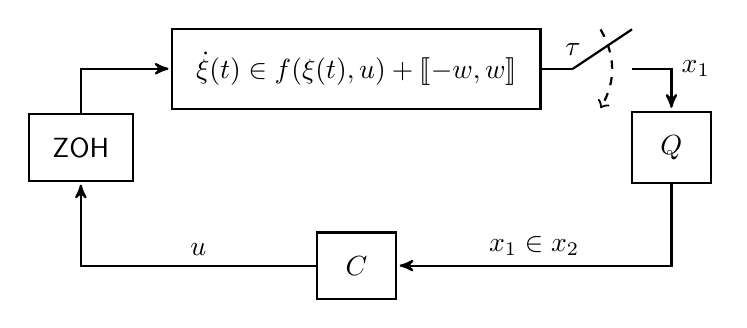
\begin{tikzpicture}
    [
    mynode/.style={draw,
                   thick,
                   inner sep=.3cm,
                   minimum width=1cm},
    %
    to/.style={->,
               >=stealth',
               shorten >=1pt,
               thick},
    ]

    \node [mynode] (sys) at (0,0) {$\dot \xi(t)\in f(\xi(t),u)+\segcc{-w,w}$};
    \node [mynode] (con) at (0,-2.5) {$C$};
    \node [mynode] (zoh) at (-3.5,-1) {$\mathsf{ZOH}$};

    %\node [mynode] (dist) at (4,0) {$P$};
    \node [mynode] (quant) at (4,-1) {$Q$};

    \node at (2.75,0.25) {$\tau$};


    \draw [to]  (zoh.north) |-  (sys.west);
    \draw [to]  (con.west)  -| node[above, near start] {$u$} (zoh.south);

    \draw[to] (3.5,0) -| node[right] {$x_1$} (quant.north);
    \draw[to] (quant.south) |- node[above, near end] {$x_1\in x_2$} (con.east);

    \draw[thick] (sys.east) -- (2.75,0);
    \draw[thick] (2.75,0) -- (3.5,.5);
    \draw[dashed,thick,bend left,->] (3.1,.5) to (3.1,-.5);

  \end{tikzpicture}
\caption{Sample-and-hold implementation of a controller synthesized with {\tt SCOTS}.}\label{f:closedloop}
\end{figure}

%In case that
%$\Sigma_1$ is an invariance or a reachability specification, the solution $C$ is
%a \emph{static} system, which means that the state alphabet is a singleton, i.e.,
%$X_c=\{x_c\}$. The output function 
%
%In the simplest
%case, $C$ is a \emph{static} system, which means $X_c$

Additionally to the perturbations on the right-hand-side
of~\eqref{e:sys:ct}, it is possible to account for measurement errors
modeled by a set-valued map $P \colon \mathbb{R}^n \rightrightarrows
\mathbb{R}^n$ given by
\begin{IEEEeqnarray}{c't'c}\label{e:perturbation}
  P(x):=x+\segcc{-z,z} & with & z\in\R_+^n.
\end{IEEEeqnarray}
Please see~\cite[Sec.~VI.B]{ReissigWeberRungger15} and~\cite{RunggerZamani16}
for some background theory.
The closed loop with measurement errors is illustrated
in~Fig.~\ref{f:closedloop:pert}.
\begin{figure}[h]
\centering
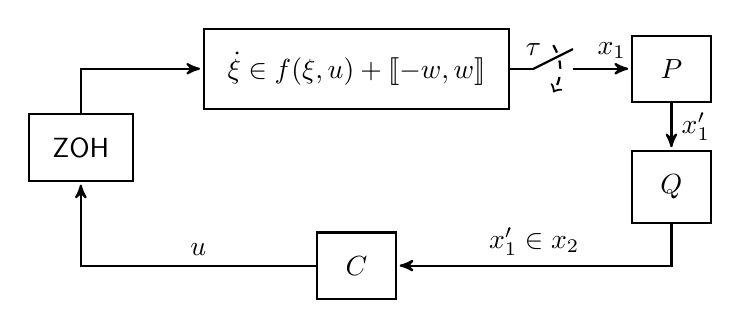
\begin{tikzpicture}
  [
  mynode/.style={draw,
                 thick,
                 inner sep=.3cm,
                 minimum width=1cm},
  %
  to/.style={->,
             >=stealth',
             shorten >=1pt,
             thick},
  ]

  \node [mynode] (sys) at (0,0) {$\dot \xi\in f(\xi,u)+\segcc{-w,w}$};
  \node [mynode] (con) at (0,-2.5) {$C$};

  \node [mynode] (zoh) at (-3.5,-1) {$\mathsf{ZOH}$};

  \node [mynode] (dist) at (4,0) {$P$};
  \node [mynode] (quant) at (4,-1.5) {$Q$};

  \node at (2.25,0.25) {$\tau$};


  \draw[thick] (sys.east) -- (2.25,0);
  \draw[thick] (2.25,0) -- (2.75,.25);
  \draw[dashed,thick,bend left,->] (2.5,.3) to (2.5,-.3);
  \draw[thick] (2.75,0) -- (3,0);

  \draw[to] (3,0) -- node[above] {$x_1$} (dist.west);
  \draw[to] (dist.south) -- node[right] {$x_1'$} (quant.north);


  \draw [to]  (zoh.north) |-  (sys.west);
  \draw [to]  (con.west)  -| node[above, near start] {$u$} (zoh.south);

  \draw[to] (quant.south) |- node[above, near end] {$x'_1\in x_2$} (con.east);

\end{tikzpicture}
\caption{Closed loop with measurement errors modeled by the set-valued map $x'_1 \in P(x_1)$.}\label{f:closedloop:pert}
\end{figure}

\section{Construction of Symbolic Models}

\subsection{Growth Bound and A Priori Enclosure}
\label{ss:GB} 

The construction of a symbolic model $S_2$ of $S_1$
is based on the over-approxima\-tion of
attainable sets. In {\tt SCOTS}, the over-approximation of the attainable sets
requires a so-called growth bound~\cite{ReissigWeberRungger15}.
A \emph{growth bound} of~\eqref{e:sys:ct} is a function $\beta \colon
\mathbb{R}_{+}^n \times U' \to \mathbb{R}_{+}^n$, which is defined with respect to a sampling time
$\tau>0$, a set $K\subseteq \mathbb{R}^n$ and a set $U'\subseteq U$.
Basically, it provides an upper bound on the deviation of solutions $\xi$
of~\eqref{e:sys:ct} from \emph{nominal
solutions}\footnote{A nominal solution $\varphi(\cdot,p,u)$ of
\eqref{e:sys:ct} is defined as solution of the initial value problem $\dot x=f(x,u)$,
$x(0)=p$.} $\varphi$ of~\eqref{e:sys:ct}, i.e., for every solution $\xi$ of \eqref{e:sys:ct} on $\intcc{0,\tau}$ with input $u \in U'$ and $\xi(0),p \in K$,
we have
\begin{IEEEeqnarray}{c}
\label{e:growthbound}
| \xi(\tau) - \varphi(\tau,p,u) | \leq \beta( | \xi(0) - p |, u).
\end{IEEEeqnarray}
Here, $|x|$ for $x\in\R^n$, denotes the component-wise absolute value.
A growth bound can be obtained essentially by bounding
the Jacobian of $f$. Let
$L \colon U' \to \mathbb{R}^{n \times n}$ satisfy
\begin{IEEEeqnarray}{c}\label{e:lipschitz}
L_{i,j}(u)
\geq
\begin{cases}
D_j f_i(x,u)& \text{if $i=j$,}\\
| D_j f_i(x,u) |& \text{otherwise}
\end{cases}
\end{IEEEeqnarray}
for all $x\in K'\subseteq \R^n$ and $u\in U'\subseteq U$. Then 
\begin{IEEEeqnarray}{c}
\label{e:GrowthBoundComputation}
\beta(r,u)
=
e^{L(u)\tau}
r
+
\int_0^\tau
e^{L(u)s}
w
\;\mathrm{d}s,
\end{IEEEeqnarray}
is a growth bound on $\intcc{0,\tau}$, $K$, $U'$
associated with \eqref{e:sys:ct}. The set $K'$ on
which~\eqref{e:lipschitz} needs to hold, is a so-called \emph{a priori
enclosure}, i.e., $K'$  is assumed to be convex and contain any
solution $\xi$ on $\intcc{0,\tau}$ of~\eqref{e:sys:ct} with $u\in U'$ and
$\xi(0)\in K$,
see~\cite[Thm.~VIII.5]{ReissigWeberRungger15}. 

In order to use {\tt SCOTS}, the user needs to provide a growth bound, which for
nonlinear control systems can be provided in terms of the parameterized matrix
$L(u)$ whose entries satisfy~\eqref{e:lipschitz}. A priori enclosures as well
as growth bounds can be computed automatically using interval arithmetic based
ODE solvers. See Section~\ref{s:usage:abs} for more details on how to
automatically obtain a priori enclosures and growth bounds.
%An implementation of such computations using the interval ODE
%solver {\tt vnodelp} for the aircraft example can be found in the directory
%\begin{lstlisting}[basicstyle=\small\ttfamily]
%./examples/aircraft/helper        	
%\end{lstlisting}


\subsection{The Transition Function}

Recall that the state alphabet $X_2$ of the symbolic model $S_2=(X_2,U_2,F_2)$
is composed of the real quantizer symbols $\bar X_2$, which are cells aligned on a
uniform grid, and the overflow symbols $X_2\smallsetminus \bar X_2$. For $x_2\in
X_2\smallsetminus \bar X_2$ the transition function is defined for all $u\in
U_2$ by
\begin{IEEEeqnarray}{c}
  F_2(x_2,u):=\emptyset.
\end{IEEEeqnarray}
In order to determine the successors $x_2'\in F_2(x_2,u)$ for 
$x_2=c+\segcc{-\eta/2,\eta/2}\in \bar X_2$ and $u\in U_2$, we first compute the
hyper-interval 
\begin{IEEEeqnarray}{c}\label{e:theory:attainableset}
  R:=\varphi(\tau,c,u)+\segcc{-\beta(\eta/2,u),\beta(\eta/2,u)}
\end{IEEEeqnarray}
which is an over-approximation of the attainable set of~\eqref{e:sys:ct}
with respect to the set $c+\segcc{-\eta/2,\eta/2}$ and input $u$.
If $P$ is not covered by the real quantizer symbols, i.e.,  $R\not\subseteq
\cup_{x_2\in \bar X_2} x_2$, then we define
\begin{IEEEeqnarray}{c}
  F_2(x_2,u):=\emptyset.
\end{IEEEeqnarray}
Otherwise, we define the successor cells function by
\begin{IEEEeqnarray}{c}\label{e:theory:tf3}
x_2'\in F_2(x_2,u):\iff x_2'\cap R\neq\emptyset.
\end{IEEEeqnarray}
Using similar arguments as in~\cite[Thm.~VIII.4]{ReissigWeberRungger15}, it is
straightforward to show that $Q$ is a feedback refinement relation from $S_1$ to
$S_2$. Note that $F_2$ satisfies 
\begin{IEEEeqnarray}{c}\label{e:theory:tf4}
 F_2(x_2,u)\subseteq \bar X_2.
\end{IEEEeqnarray}

If we need to be robust against measurement errors $P(x)=x+\segcc{-z,z}$, we
slightly modify the computation of $R$ to 
\begin{IEEEeqnarray}{c}
  R:=\varphi(\tau,c,u)+\segcc{-\beta(\eta/2+z,u),\beta(\eta/2+z,u)}
\end{IEEEeqnarray}
and define the transition function to (instead of~\eqref{e:theory:tf3})
\begin{IEEEeqnarray}{c}
x_2'\in F_2(x_2,u):\iff (x_2'+\segcc{-z,z})\cap R\neq\emptyset.
\end{IEEEeqnarray}
As a result we obtain that $Q\circ P$ is a feedback refinement relation from
$S_1$ to $S_2$, see~\cite[Thm.~III.5]{WeberRunggerReissig17}, which enables the
correct controller refinement under measurement errors~\cite[Sec.~VI.B]{ReissigWeberRungger15}. The use of the
perturbation parameter $z\in\R_{>0}^n$ in {\tt SCOTS} is explained in detail in 
Section~\ref{s:usage:abs}.

In the implementation of the computation of $F_2$ in {\tt AbstractionGB.hh}, we use a numerical ODE solver
to compute an approximation of $\varphi(\tau,c,u)$ as well as $\beta(\eta/2,u)$.

\section{Controller Synthesis}
\label{s:theory:alg}

We discuss the algorithms that are implemented in {\tt SCOTS} to
solve synthesis problems for the finite symbolic model $S_2=(X_2,U_2,F_2)$. 
We use the following notation. The set of \emph{admissible inputs} at $x_2\in X_2$ is denoted by
\begin{IEEEeqnarray}{c}
U_{S_2}(x_2):=\{u\in U_2\mid F_2(x_2,u)\neq\emptyset\}.
\end{IEEEeqnarray}
We use the Weierstrass symbol $\wp$ to denote the power set and define $\pre:\wp(X_2)\to \wp(X_2)$ by
\begin{IEEEeqnarray}{c}\label{e:pre}
  \pre(Y):=\{x_2\in X_2\mid  \exists_{u\in U_{S_2}(x_2)}:\;F_2(x_2,u)\subseteq Y\}.
\end{IEEEeqnarray}

Usually, synthesis algorithms are developed in the context of two-player games on graphs. The player associated with the controller tries to
enforce the specification while the player associated with disturbances tries to
violate the specification, e.g.~\cite{BloemJobstmannPitermanPnueliSaar12}.


\subsection{Invariance}

Let $\Sigma_2$ be an invariance specification associated with $I_2$ and $Z_2$. 
We use Alg.~\ref{a:safety}, which is implemented in the function {\tt
solveInvarianceGame} in the file {\tt GameSolver.hh}, to synthesize a controller
that solves the control problem $(S_2,\Sigma_2)$.  
Alg.~\ref{a:safety} runs in $O(m)$ time, where $m$ is the number of transitions, i.e., the number of
triples $(x_2,u,x'_2)$ with $x'_2\in F_2(x_2,u)$, since each state is added to the queue
of bad states $Q$ at most once.

\begin{algorithm}[h]
\caption{Controller synthesis for invariance specs associated with $I_2$ and $Z_2$}\label{a:safety}
  \begin{algorithmic}[1]
    \Input{$Z_2$, $S_2=(X_2,U_2,F_2)$}
    \Require{$F_2(X_2,U_2)\subseteq \bar X_2$ and $Z_2\subseteq \bar X_2$}
    \State $Q:=\emptyset$ \Comment{ FIFO queue of bad states} 
    \State $E:=\emptyset$ \Comment{ bookkeeping of the bad states} 
    \State $D:=\emptyset$ \Comment{ valid state-input pairs}
    \ForAll{$x_2\in \bar X_2$}
    \If{$x_2\not\in Z_2$ or $U_2(x_2)=\emptyset$}
    \Comment{ mark all states outside $Z_2$ or blocking states as bad}
    \State $Q:=Q\cup \{x_2\}$
    \Else 
    \State $D:=D\cup (\{x_2\}\times U_2(x_2))$ 
    \EndIf
    \EndFor
    \State $E:=Q$
    \While{ $Q\neq\emptyset$ }
    \State $x'_2:\in Q$ \Comment{remove oldest element}\label{a:safety:beginwhile}
    \State $Q:=Q\smallsetminus \{x_2'\}$\label{a:safety:remQ}
    \ForAll{$(x_2,u)\in F_2^{-1}(x_2')$}
    \State $D:=D\smallsetminus \{(x_2,u)\}$\label{a:safety:remove}
    \Comment{ remove state-input pairs that lead to bad states}
    \If{$x_2\not \in D^{-1}(U_2)$ and $x_2\not\in E$}
    \Comment{ no valid input left and not already marked bad}
    \State $Q:=Q\cup\{x_2\}$\label{a:safety:addQ}
    \Comment{ add to queue of bad states}
    \State $E:=E\cup\{x_2\}$\label{a:safety:addE}
    \EndIf
    \EndFor
    \EndWhile
    \Output $D$
  \end{algorithmic}

\end{algorithm}

Let $D\subseteq X_2\times U_2$ be the set of state-input pairs computed in
Alg.~\ref{a:safety}. One can show that $D^{-1}(U_2)$ is the \emph{maximal fixed
point} of the map $G:\wp(X_2)\to \wp(X_2)$ defined by
\begin{IEEEeqnarray}{c}\label{e:theory:fp:safety}
  G(Y):=Z_2\cap\pre(Y).
\end{IEEEeqnarray}
The maximal fixed point of~\eqref{e:theory:fp:safety}
characterizes the largest set of initial states from which the invariance
condition can be enforced and it follows that the synthesis problem $(S_2,\Sigma_2)$ is solvable if and only
if $I_2\subseteq D^{-1}(U_2)$. 

%\begin{lemma}
%Let $S_2=(X_2,U_2,F_2)$ be a finite simple system with $\bar X_2\subseteq X_2$
%and $F_2(X_2,U_2)\subseteq \bar X_2$. Let $Z_2\subseteq \bar X_2$ and let $D$ be the output of
%Alg.~\ref{a:safety}. The set $Y_\infty:=D^{-1}(U_2)$ is the maximal fixed point
%of~\eqref{e:theory:fp:safety}.
%\end{lemma}
%\begin{proof}
%Let $D_i$, $E_i$ and $Q_i$ denote the sets $D$, $E$ and $Q$
%manipulated in Alg.~\ref{a:safety} at the beginning of the while loop in
%line~\ref{a:safety:beginwhile} of iteration $i\in \Z_{\ge0}$. For example for
%$i=0$ we have $D_0=\{(x,u) \mid x\in Z_2\wedge u\in U_{S_2}(x)\}$ and $D_{i+1}$
%results from $D_i$ by removing the elements in line~\ref{a:safety:remove}.
%Similarly, $E_0=Q_0$ and $E_{i+1}$ results from $E_i$ by adding elements in
%line~\ref{a:safety:addE} and $Q_{i+1}$ results from $Q_i$ by adding and removing
%elements in line~\ref{a:safety:addQ} and line~\ref{a:safety:remQ}, respectively.
%Parallel to $D_i$ we introduce $Y_i:=D_i^{-1}(U_2)$.  Let us point out that for
%all $i\ge0$ we have $Q_i\subseteq E_i$, $E_i=\cup_{i'\in\intcc{0;i}} Q_{i'}$ and the sets 
%$E_i$ and $Y_i$ are disjoint and satisfy $\bar X_2=E_i\cup Y_i$. Also $Y_{i+1}\subseteq Y_i\subseteq \cdots
%\subseteq Z_2$ and there exists $i^*\in \Z_{\ge0}$ so that $Y_{i^*}=Y_\infty$.
%
%Let us first show that $Y_\infty=G(Y_\infty)$. Let $Y_\infty
%=Y_{i^*}$ and $x\in Y_{i^*}$. Since $Y_{i^*}\subseteq Z_2$ we have $x\in Z_2$
%and it remains to show that $x\in \pre(Y_{i^*})$. Let
%$u\in U_{S_2}(x)$ be such that $(x,u)\in D_{i^*}$. As $(x,u)\in D_{i^*}$ we
%conclude $F(x,u)\cap Q_i=\emptyset$ for all $i\in\intcc{0;i^*}$ (otherwise
%$(x,u)$ would have been removed in line~\ref{a:safety:remove}). We obtain
%$F(x,u)\cap E_{i^*}=\emptyset$. Since $F_2(x,u)\subseteq \bar X_2$ and $\bar
%X_2=E_{i^*}\cup Y_{i^*}$ it follows that $F_2(x,u)\subseteq Y_{i^*}$ and $x\in
%\pre(Y_{i^*})$ follows.  Now let $x\in G(Y_{i^*})=Z_2\cap \pre(Y_{i^*})$ and
%assume for the sake of contradiction that $x\not\in Y_{i^*}$.
%Let $u\in U_{S_2}(x)$ so that $F_2(x,u)\subseteq Y_{i^*}$. Since
% $x\in Z_2$ we see that $(x,u)\in D_0$. Hence, if $x\not\in Y_{i^*}$ all pairs $(\bar x,\bar u)$
%with $\bar x=x$ (including the pair $(x,u)$) need to have been removed from $D_0$ along the iteration
%$i\in\intcc{0;i^*}$. However, from $F_2(x,u)\subseteq Y_{i^*}$ follows that
%$F_2(x,u)\cap E_{i^*}=\emptyset$. Moreover, 
%for all $i\in\intcc{0;i^*}$ holds $Q_i\subseteq E_{i^*}$ and we obtain $F_2(x,u)\cap
%  Q_{i}=\emptyset$ for all $i\in\intcc{0;i^*}$ so that we arrive at a contradiction
%  since $(x,u)$ cannot have been removed from $D_0$ in line~\ref{a:safety:remove}.
%
%Let $\bar Y\subseteq X_2$. We show that $\bar Y \subseteq G(\bar Y)$ implies
%$\bar Y\subseteq Y_\infty$ by induction over  $i\ge 0$.
%Let $i=0$ and $x\in \bar Y$. Since
%$\bar Y\subseteq G(\bar Y)$ we have $x\in Z_2$ and $U_{S_2}(x)\neq\emptyset$,
%which shows that $x\in Y_0$. Now suppose that $\bar Y\subseteq Y_i$ but $\bar
%Y\not\subseteq Y_{i+1}$, i.e., there exist $x\in (Y_i\smallsetminus Y_{i+1})\cap
%\bar Y$. That means all pairs $(\bar x,\bar u)$ with $\bar x=x$ in $D_i$ have been removed in line~\ref{a:safety:remove}. 
%However, there exists at least one $u\in U_{S_2(x)}$ with
%$F_2(x, u)\cap Q_i=\emptyset$. That follows from
%the fact that $x\in G(\bar Y)$, $\bar Y\subseteq Y_i$ and $Q_i\cap Y_i\neq
%\emptyset$. Hence,
%we obtain a contradiction and $\bar Y\subseteq Y_{i+1}$ follows. As this holds
%for all $i\ge0$ we conclude that $\bar Y\subseteq Y_{\infty}$ and the assertion follows.
%\end{proof}


Suppose that $I_2\subseteq D^{-1}(U_2)$ holds, then we obtain a controller
$C=(\{q\},\{q\},X_2,X_2,U_2,F_c,H_c)$
that solves $(S_2,\Sigma_2)$ by  
\begin{IEEEeqnarray}{rCl}\label{e:controller}
\begin{IEEEeqnarraybox}[][c]{rCl}
H_c(q,x_2)&=&
\begin{cases}
D(x_2)\times \{x_2\} & \text{if } x_2\in D^{-1}(U_2)\\
U_2\times\{x_2\} & \text{otherwise}
\end{cases}\\
F_c(q,x_2)&=&
\begin{cases}
\{q\} & \text{if } x_2\in D^{-1}(U_2)\\
\emptyset &  \text{otherwise.}
\end{cases}
\end{IEEEeqnarraybox}
\end{IEEEeqnarray}
The refined controller $C\circ Q$ that is feedback composed with $S_1$ is
implemented in {\tt SCOTS} in the {\tt StaticController} class. The details are
explained in Section~\ref{s:usage:simulation}.


\subsection{Reachability}

Let $\Sigma_2$ be a reachability specification associated with $I_2$ and
$Z_2\subseteq \bar X_2$. 
We use Alg.~\ref{a:reach}, which is implemented in the function 
{\tt solveReachabilityGame} in the file {\tt GameSolver.hh}, to synthesize a controller
that solves the control problem $(S_2,\Sigma_2)$. The algorithm is a variant of
Dijkstra's shortest path algorithm for hyper-graphs taken
from~\cite{GalloLongoPallotinoNguyen93}. It runs in $O(m)$ time, where $m$ is
the number of transitions, i.e., the number of elements in $X_2\times U_2\times
X_2$ that satisfy $x_2'\in F_2(x_2,u)$.

\begin{algorithm}[h]
  \caption{Controller synthesis for reachability specs associated with $I_2$ and $Z_2$}
  \label{a:reach}
  \begin{algorithmic}[1]
    \Input{ $Z_2$, $S_2=(X_2,U_2,F_2)$, $u_0\in U_2$}
    \Require{ $Z_2\subseteq \bar X_2$}
    \State {$Q := Z_2$ \Comment{FIFO queue}}
    \State {$V := \infty$}\Comment{value function}\label{a:reach:initV}
    \State $M:=0$ \Comment{intermediate values} 
    \State {$E := \emptyset$ \Comment{bookkeeping of processed states}}
    \ForAll {$x_2 \in\bar X_2$}
      \State {$D(x_2) := \emptyset$}\Comment{keep track of optimal input}
      \If{$x_2\in Z_2$}
        \State {$V(x_2) := 0$}\Comment{cost at target are zero}
        \label{a:reach:setV}
        \State {$D(x_2) := \{u_0\}$}\label{a:reach:initD}
        \label{a:reach:initD}
      \EndIf
    \EndFor
    \While {$Q \not= \emptyset$}
      \State {$x_2' :\in  Q $} \Comment{remove oldest element} \label{a:reach:remove}
      \State {$Q := Q \smallsetminus \{ x_2' \}$}
      \State {$E := E \cup \{ x_2' \}$}\label{a:reach:addE}
      \ForAll {$(x_2,u) \in F_2^{-1}(x_2')$}
        \State $M(x_2,u):=\max\{M(x_2,u),V(x_2')\}$
        \If {$F_2(x_2,u) \subseteq E$ and $V(x_2) > 1+M(x_2,u)$} \Comment{if $u$ leads to better cost update input}
        \label{a:reach:conditions}
          \State {$V(x_2) := 1+M(x_2,u)$} \label{a:reach:updateV}
          \State {$Q := Q \cup \{ x_2 \}$}\label{a:reach:add}
          \State {$D(x_2) := \{ u \}$}\label{a:reach:setD}
        \EndIf
      \EndFor
    \EndWhile
    \Output {$D$, $V$}
  \end{algorithmic}
\end{algorithm}

Let $D$ be the output of Alg.~\ref{a:reach}.
The set $D^{-1}(U_2)$ is
the \emph{minimal fixed point} of the map $G:\wp(X_2)\to \wp(X_2)$ defined by
\begin{IEEEeqnarray}{c}\label{e:theory:fp:reach}
  G(Y):=Z_2\cup\pre(Y).
\end{IEEEeqnarray}
The minimal fixed point of~\eqref{e:theory:fp:reach} characterizes the largest
set from which every element of the behavior of the system $S_2$ can be forced
to reach the set $Z_2$.
It follows that the synthesis problem $(S_2,\Sigma_2)$ is solvable if and only
if $I_2\subseteq D^{-1}(U_2)$. 

%\begin{lemma}
%Let $S_2=(X_2,U_2,F_2)$ be a finite simple system with $\bar X_2\subseteq X_2$,
%let $Z_2\subseteq \bar X_2$  and let $D$ be the output of
%Alg.~\ref{a:reach}. Then $Y_\infty:=D^{-1}(U_2)$ is the minimal fixed point
%of~\eqref{e:theory:fp:reach}.
%\end{lemma}
%\begin{proof}[Proof sketch]
%Let $Q_i$ denote the set $Q$ that is processed Alg.~\ref{a:reach} at iteration
%$i$ of the while loop in line~\ref{a:reach:remove}. For example $Q_0=Z_2$ and
%$Q_{i+1}$ results from $Q_i$ by removing and adding elements in
%line~\ref{a:reach:remove} and~\ref{a:reach:add}, respectively. Let $i^*$ denote
%the iteration when the algorithm terminates, i.e., $Q_{i^*}=\emptyset$. Since
%every element of $Q_i$ for all $i\in\intco{0;i^*}$ is added to $E$ in
%line~\ref{a:reach:addE}, we have 
%$E=\cup_{i\in\intcc{0;i^*}}Q_i$. Moreover, $D(x)\neq\emptyset$ holds iff 
%$x\in Q_i$ for some $i\in\intco{0;i^*}$ and we see that $Y_\infty=E$.
%Another invariant which is easy to check is: $x\in Q_i$ for some $i\in
%\intco{0;i^*}$ implies $V(x)<\infty$. Hence $M(x,u)$ is finite for every
%$(x,u)\in X_2\times U_2$ throughout the whole computation.
%
%Let us show that $Y_\infty$ is a fixed point of~\eqref{e:theory:fp:reach}.
%Let $x\in Y_\infty$. If $x\in Z_2$ we immediately obtain $x\in G(Y_\infty)$.
%For $x\not\in Z_2$ we see that $D(x)$ has been set in line~\ref{a:reach:setD}
%and we obtain $F_2(x,D(x))\subseteq E=Y_\infty$. Now let $x\in G(Y_\infty)$. If
%$x\in Z_2$ we use line~\ref{a:reach:initD} to infer $x\in Y_\infty$ and
%subsequently we consider $x\in \pre(Y_\infty)$. Since $Y_\infty=E$, there exists
%$u\in U_{S_2}(x)$ so that $F_2(x,u)\subseteq E$. Since $M(x,u)<\infty$ holds
%throughout the computation and initially $V(x)=\infty$, we see that there must have been an iteration $i$ where
%both conditions in line~\ref{a:reach:conditions} have been true for $(x,u)$ (in
%place of $(x_2,u)$), so that
%$D(x)\neq\emptyset$, which shows $x\in Y_\infty$.
%
%We continue to show that $Y_\infty$ is the minimal fixed point
%of~\eqref{e:theory:fp:reach}.
%Let $D_i$ denote the map $D$ computed in Alg.~\ref{a:reach} at
%line~\ref{a:reach:remove}, i.e., $D_0$ is
%computed in line~\ref{a:reach:initD} and $D_{i+1}$ results from $D_i$ by setting
%the input in line~\ref{a:reach:setD}. Let $Y_i:=D_i^{-1}(U_2)$ and observe that
%$Y_0=Z_2$ and $Y_i\subseteq Y_{i+1}$ holds for all $i\ge0$. One can also show
%that $Y_{i+1}\subseteq G(Y_i)$.
%Moreover, one can show that $G$ is monotone, i.e., for  $Y,Y'\subseteq \bar X_2$ the inclusion
%$Y\subseteq Y'$ implies $G(Y)\subseteq G(Y')$. Given this fact it is easy to see
%that $G(\bar Y)\subseteq \bar Y$ implies $Y_{i}\subseteq \bar Y$ for all $i\ge0$, since we
%have $Y_0=Z_2\subseteq \bar Y$ and $Y_{i+1}\subseteq G(Y_i)\subseteq G(\bar
%Y)\subseteq \bar Y$. Given that the algorithm terminates there exists $i^*$ with
%$Y_\infty=Y_{i^*}$ and $Y_\infty\subseteq \bar Y$ follows.
%\end{proof}

Given that $I_2\subseteq D^{-1}(U_2)$ holds, a controller
$C=(\{q\},\{q\},X_2,X_2,U_2,F_c,H_c)$ that solves $(S_2,\Sigma_2)$ is identical
to the controller that solves the invariance problem, i.e., $F_c$ and $H_c$ are
given by~\eqref{e:controller}.

Again, the refined controller $C\circ Q$ that is feedback composed with $S_1$ is
implemented in {\tt SCOTS} in the {\tt StaticController} class. The details are
explained in Section~\ref{s:usage:simulation}.

\subsection{Reach-Avoid}
Let $\Sigma_2$ be a reach-avoid specification associated with $I_2$ and $A_2,Z_2\subseteq \bar X_2$. 
{\tt SCOTS} provides two alternatives on how to synthesize controller to enforce
reach-avoid specifications. In the first method, the avoid set $A_2$ is
accounted for in the transition function, i.e.,
\begin{IEEEeqnarray}{c'c}\label{e:theory:tf:avoid}
  \forall_{x_2\in A_2}:& F_2(x_2,u):=\emptyset.
\end{IEEEeqnarray}
In this way we can reduce a reach-avoid problem to a reachability problem. 
Given that the transition function satisfies \eqref{e:theory:tf:avoid}, any
controller that solves the control problem $(S_2,\Sigma_2')$, where $\Sigma_2'$
is the reachability specification associated with $I_2$ and $Z_2$, also solves the
control problem $(S_2,\Sigma_2)$. In order to enforce the
equation~\eqref{e:theory:tf:avoid} in the computation of the transition function
$F_2$ the user can optionally supply the avoid set to the function {\tt
AbstractionGB::computeTransitionRelation}, see Section~\ref{s:usage:abs}.

For the second method, the computation of the transition function is left
unchanged, but Alg.~\ref{a:reach} is modified to account for the avoid set. To
this end the condition in line~\ref{a:reach:conditions} in Alg.~\ref{a:reach} is modified to 
\begin{IEEEeqnarray}{c't'c't'c}\label{a:avoid}
 F_2(x_2,u) \subseteq E& and &V(x_2) > 1+M(x_2,u)& and & x_2\not\in A_2.
\end{IEEEeqnarray}
Again the user can optionally supply the avoid set to the function {\tt
solveReachabilityGame}, see Section~\ref{s:usage:synthesis}.


%\subsection{Customized Synthesis Algorithms}
%\label{s:theory:customized}
%
%Even though {\tt SCOTS} natively supports only invariance and reachability
%specification, an advanced user has the possibility to write customized
%synthesis algorithms. We demonstrate such a customization for persistence and
%recurrence specifications. 
%
%Let $S=(X,U,F)$ be a finite simple
%system with and consider the sets $I, Z, T_i\subseteq X$, $i\in\intcc{1;p}$,
%$p\in\N$. The \emph{persistence} specification $\Sigma$ for $S$ associated with $I$ and $Z$ is given by
%\begin{IEEEeqnarray}{c}
%  \Sigma:=\big\{(u,x)\in (U\times X)^\infty
%  \mid  x(0)\in I\implies 
%    \exists_{t\in\intco{0;\infty}}\forall_{t'\in\intcc{t;\infty}}: x(t')\in Z
%  \big\}.
%\end{IEEEeqnarray}
%The \emph{recurrence} specification $\Sigma$ for $S$ associated with $I$ and
%$T_i$, $i\in\intcc{1;p}$, $p\in\N$ is given by
%\begin{IEEEeqnarray}{c}
%  \Sigma:=\big\{(u,x)\in (U\times X)^\infty
%  \mid  x(0)\in I\implies 
%    \forall_{t\in\intco{0;\infty}}\forall_{i\in\intcc{1;p}}\exists_{t'\in\intcc{t;\infty}}:
%    x(t')\in T_i
%  \big\}.
%\end{IEEEeqnarray}
%Using the $\mu$-calculus notation, e.g. used
%in~\cite{BloemJobstmannPitermanPnueliSaar12}, to denote minimal and maximal fixed
%points of monotone functions, we can characterize the set of \emph{winning
%states} for persistence and recurrence specifications by the fixed point expressions
%\begin{IEEEeqnarray}{c}
%  \mu Y_1.\nu Y_2. \pre(Y_1)\cup (\pre(Y_2)\cap Z)
%\end{IEEEeqnarray}
%respectively
%\begin{IEEEeqnarray}{c}
%  \nu Y_1.\bigcap_{i\in\intcc{1;p}}\mu Y_2. \pre(Y_2)\cup (\pre(Y_1)\cap T_i).
%\end{IEEEeqnarray}




\newpage


\part{USAGE}

\section{Computation of Symbolic Models}
\label{s:usage:abs}

Let $S_1=(X_1,U_1,F_1)$ be a simple system that represents the $\tau$-sampled
behavior of continuous-time system~\eqref{e:sys:ct} as defined in
Section~\ref{s:theory:control_problems}. In order to compute a symbolic model
$S_2=(X_2,U_2,F_2)$ of $S_1$, i.e., the relation $Q$ in~\ref{e:theory:quantizer} is a feedback
refinement relation from $S_1$ to $S_2$, the following ingredients are needed:
\begin{enumerate}
  \item the set of real quantizer symbols $\bar X_2$;
  \item the input alphabet $U_2$;
  \item the solution $\varphi(\tau,p,u)$ of the IVP $\dot \xi = f(\xi,u)$,
  $\xi(0)=p$ at time $\tau$;
  \item a growth bound $\beta(r,u)$.
\end{enumerate}
Subsequently, we demonstrate the usage of {\tt SCOTS} to compute a symbolic
model of the $\tau$-sampled aircraft dynamics used
in~\cite[Sec.~IX.B]{ReissigWeberRungger15}. 

First, we define the set of real quantizer symbols $\bar X_2$ (defined
in~\eqref{e:theory:ss}) and the input
alphabet $U_2$. To this end, {\tt SCOTS} provides the class {\tt UniformGrid}. T  parameterized by the
grid parameter $\eta\in \R^n_{>0}$ and the confining vectors  $a,b\in \R^n$. An
instance is created by

\section{Controller Synthesis}
\label{s:usage:synthesis}

\section{Closed Loop Simulation}
\label{s:usage:simulation}
The
function {\tt StaticController::control} takes as input a state $x_1\in X_1$ and
rounds it to the nearest grid point in $\eta\Z$ in order to determine a
symbolic state $x_2\in Q(x_1)$. If there does not exist a valid input $u\in U_2$
associated with $x_2$, i.e., $x_2\not\in \pi_{X_2}(D)$, then the
$F_c(q,x_2)=\emptyset$ and function returns the error message
\begin{lstlisting}[basicstyle=\small\ttfamily]
scots::StaticController::control: no progress possible at state <values> 
\end{lstlisting}
Otherwise, {\tt StaticController::control} returns the set of valid control
inputs.



\section{Writing To and Reading From Hard Disk}

\section{MATLAB Interface}

\section{Customized Synthesis Algorithms}


\newpage



\subsection{Symbolic Set}
Each instance of the \Cpp class {\tt\small SymbolicSet}, whose source code is
located in {\tt\small ./bdd/SymbolicSet.hh}, is associated with a \emph{domain}
$\segcc{a,b}\subseteq \R^n$ and a \emph{grid parameter} $\eta\in \R_{>0}^n$. The class is used to create,
manipulate and store a \emph{subset} of the grid points contained in
\begin{IEEEeqnarray*}{c}
  D:=(\intcc{a_1,b_1}\times \cdots\times \intcc{a_n,b_n} )\cap  \eta\Z^n.
\end{IEEEeqnarray*}
Each grid point $x\in D$ is identified with a cell $x+\segcc{-\eta/2,\eta/2}$. Throughout the reminder of this section, let us use 
\begin{IEEEeqnarray*}{c}
 S\subseteq  D
\end{IEEEeqnarray*}
to denote the subset of $D$ which is encoded by an instance of the class {\tt
\small SymbolicSet}. Each grid point $x\in D$ is defined in terms of a number of binary
decision ({\tt\small BDD}) variables $d\in\B^{m}$ created with
the {\tt CUDD} library (see~\eqref{e:mapping} for details).
%In {\tt SCOTS} an element of $d\in\B^m$ evaluates to one, i.e., $f(d)=1$ if and
%only if the grid point $x$ represented by $d$ is an element of the set $S$ represented by {\tt\small SymbolicSet}
Each {\tt \small BDD} variable obtains
a unique {\tt \small id}. The domain $\segcc{a,b}\subseteq \R^n$, grid parameter
$\eta\in \R_{>0}^n$ together with the {\tt \small BDD} variable {\tt \small id}s
associated with an instance of a {\tt\small SymbolicSet} make up the
\emph{abstract domain}.  
There exist several possibilities to instantiate an object
of the class {\tt\small SymbolicSet}:
\begin{enumerate}
  \item By using the domain $\segcc{a,b}\subseteq \R^n$ and grid parameter
    $\eta\in\R^n_{>0}$, in which case new {\tt\small BDD} variables are created.
    For example, to encode a set of grid points in $\intcc{-1,1}^2\cap
    (0.1,0.1)\Z^2$, we can use
\begin{lstlisting}[basicstyle=\footnotesize\ttfamily]
#include <array>
#include <iostream>
#include "cuddObj.hh"
#include "SymbolicSet.hh"
int main() {
  Cudd mgr;                                 /* bdd manager to organize the BDD vars */    
  double a[2]={-1,-1};                      /* lower bounds of the hyper rectangle */
  double b[2]={ 1, 1};                      /* upper bounds of the hyper rectangle */
  double eta[2]={0.1,0.1};                  /* grid node distance diameter */
  scots::SymbolicSet sset(mgr,2,a,b,eta);   /* instantiate a SymbolicSet */
  return 1;
}
\end{lstlisting}
    This is the standard instantiation method and should be used, for example, to create
    the symbolic state alphabet $\bar X_2$ and the symbolic input alphabet $U_2$, respectively.
  \item By using the copy constructor, in which case the {\tt\small BDD} variables of original
    {\tt\small SymbolicSet} instance are used for the new object.
\begin{lstlisting}[basicstyle=\footnotesize\ttfamily]
  scots::SymbolicSet nset(sset);  /* nset and sset have the same abstract domain */
\end{lstlisting}
    This option can be used for example, to create atomic propositions to
    formulate the specification. Suppose {\tt\small sset} represents $\bar X_2$,
    then we use the following code to create the {\tt\small SymbolicSet} to represent a
    subset of $\bar X_2$
\begin{lstlisting}[basicstyle=\footnotesize\ttfamily]
  scots::SymbolicSet target(sset);   /* target and sset have the same abstract domain */
\end{lstlisting}
  \item Optionally, one can specify that the {\tt\small id}'s of the {\tt\small BDD} variables should be
    newly generated
\begin{lstlisting}[basicstyle=\footnotesize\ttfamily]
  scots::SymbolicSet nset(sset,1);   /* nset and sset have different abstract domain */
\end{lstlisting}
    In this case, even though, {\tt\small nset} and {\tt\small sset} have the
    same domain $\segcc{a,b}\subseteq\R^n$ and grid parameter
    $\eta\in\R^n_{>0}$, the {\tt\small BDD} variable {\tt\small id}s are
    different and therefore, both instances {\tt\small nset} and {\tt\small sset} have a different abstract domain. 
    This instantiation method, is useful
    when it comes to the computation of the symbolic model, see
    Sec.~\ref{ss:symbolicmodelhh}.
  \item Consider two instances {\tt\small ss} and {\tt\small is} of the class
    {\tt\small SymbolicSet}, whose domains and grid parameters are given by 
    \begin{IEEEeqnarray*}{c't'c}
      \segcc{a,b}\subseteq \R^n, \eta\in \R_{>0}^n &, respectively, & \segcc{c,d}\subseteq \R^m, \mu\in \R_{>0}^m.
    \end{IEEEeqnarray*}
    Then, we can use 
\begin{lstlisting}[basicstyle=\footnotesize\ttfamily]
  scots::SymbolicSet prod(ss,is);   /* prod is the Cartesian product of ss and is */
\end{lstlisting}
   to create the object {\tt\small prod}, whose domain and grid parameter is
   given by
   \begin{IEEEeqnarray*}{c'c}
     \segcc{a,b}\times \segcc{c,d}\subseteq \R^{n+m},& (\eta,\mu)\in \R_{>0}^{n+m}.
   \end{IEEEeqnarray*}
   The {\tt\small BDD} variable {\tt\small id}s are taken from {\tt\small ss}
   and {\tt\small is}. 

   This instantiation method is useful to create a {\tt\small SymbolicSet} to
   represent the controller, see Sec.~\ref{ss:controllersynthesis}.
   

 \item Similarly, we can create an instance of {\tt\small SymbolicSet} as 
    the projection of another instance of {\tt\small SymbolicSet}. For example,
    consider the {\tt\small SymbolicSet} object  {\tt\small sset}, whose domain
    and grid parameter are given $\segcc{a,b}\subseteq \R^5$, $\eta\in \R_{>0}^5$.
    Then we use 
\begin{lstlisting}[basicstyle=\footnotesize\ttfamily]
  std::vector<size_t> pdim={1,3,4};       /* projection dimension */
  scots::SymbolicSet proj(sset,pdim); /* projection from sset onto dim {1,3,4} */
\end{lstlisting}
    to create an {\tt\small SymbolicSet} instance {\tt\small proj}, whose domain and
    grid parameter are given by
   \begin{IEEEeqnarray*}{c'c}
     \segcc{a',b'}\subseteq \R^{3},& \eta'\in \R_{>0}^{3}
   \end{IEEEeqnarray*}
   where $a'_1=a_1$, $a'_2=a_3$, $a'_3=a_4$, $b'_1=b_1$, $b'_2=b_3$, $b'_3=b_4$
   and  $\eta'_1=\eta_1$, $\eta'_2=\eta_3$, $\eta'_3=\eta_4$.
                                                 
   This instantiation method is useful to extract the {\tt\small SymbolicSet} to
   represent the state alphabet $\bar X_2$ and input alphabet $U_2$ from a {\tt\small
   SymbolicSet} which represents $\bar X_2\times U_2$, see
   Sec.~\ref{ss:symbolicmodelhh}.

\end{enumerate}                                  
                                                 
Initially, when an instance of {\tt \small SymbolicSet} is created the set $S$ is empty, i.e., it does not
contain any grid points. We can add and remove grid points associated with
polytopes and ellipsoids of the form 
\begin{IEEEeqnarray}{c't'c}\label{e:atomicprop}
  P:=\{x\in \R^n\mid Hx\le h\} & respectively & E:=\{x\in \R^n\mid |L(x-y)|_2\le 1\}
\end{IEEEeqnarray}
by using the methods
\begin{lstlisting}[basicstyle=\footnotesize\ttfamily]
SymbolicSet::addPolytope()      /* add grid points associated with a polytope to symbolicSet_ */
SymbolicSet::remPolytope()      /* remove grid points associated with a polytope from symbolicSet_ */
SymbolicSet::addEllipsoid()     /* add grid points associated with an ellipsoid to symbolicSet_ */
SymbolicSet::remEllipsoid()     /* remove grid points associated with an ellipsoid from  symbolicSet_ */
\end{lstlisting}
Each of those methods, requires an approximation parameter {\tt \small scots::INNER} or {\tt
scots::OUTER}. We use those parameters
to specify either to add an ``outer'' or ``inner'' approximation to the
{\tt\small SymbolicSet}. The inner $\check P$, $\check
E$ and outer $\hat P$, $\hat E$ approximations are given by
\begin{IEEEeqnarray*}{l'l}
  \check P :=\{x\in D\mid x+\segcc{-\eta/2,\eta/2} \subseteq P\}, 
  &
  \check E:=\{x\in D\mid |L(x-y)|_2\le 1-r\},
  \\
  \hat P :=\{x\in D\mid x+\segcc{-\eta/2,\eta/2} \cap P\neq\emptyset\},
  &
  \hat E:=\{x\in D\mid |L(x-y)|_2\le 1+r\}.
\end{IEEEeqnarray*}
where $r:=\max_{x\in\segcc{-\eta/2,\eta/2}}|Lx|_2$, which guarantees that
the following inclusions hold
\begin{IEEEeqnarray*}{c't'c}
  \bigcup_{x\in \check E} x+\segcc{-\eta/2,\eta/2}  \subseteq \big(E\cap \segcc{a,b}\big)\subseteq \bigcup_{x\in \hat E} x+\segcc{-\eta/2,\eta/2}.
\end{IEEEeqnarray*}
Further set manipulations are supported by the functions
\begin{lstlisting}[basicstyle=\footnotesize\ttfamily]
SymbolicSet::clear()            /* remove all grid points from symbolicSet_ */
SymbolicSet::addGridPoints()    /* add all grid points in the domain to symbolicSet_ */
SymbolicSet::addByFunction()    /* add grid points according to function a to  symbolicSet_ */
SymbolicSet::complement()       /* invert the grid point selection in symbolicSet_ */
\end{lstlisting}

Let us demonstrate the usage by an example.
Suppose we want to store grid points associated with a polytope and an
ellipsoid as defined in~\eqref{e:atomicprop} with 
$H\in \R^{3\times 2}$, $h\in\R^3$, $L\in \R^2$ and $y\in \R^2$ given by 
\begin{IEEEeqnarray*}{l'l'l'l}
H:= \left(
      \begin{IEEEeqnarraybox*}[][c]{,r/r,}
          1 & 0 \\ -1 & 1 \\ -1 & -1%
      \end{IEEEeqnarraybox*}
    \right), &
h:= \left(
      \begin{IEEEeqnarraybox*}[][c]{,r,}
        0 \\ .7 \\ .7%
      \end{IEEEeqnarraybox*}
    \right), &
L:= \left(
      \begin{IEEEeqnarraybox*}[][c]{,r/r,}
        2 & 0 \\ 0 & 4%
      \end{IEEEeqnarraybox*}
    \right), &
y:= \left(
      \begin{IEEEeqnarraybox*}[][c]{,r,}
        .6 \\ .25%
      \end{IEEEeqnarraybox*}
    \right).
\end{IEEEeqnarray*}
The sets are illustrated in Fig.~\ref{f:symbolicset} on the left.
\begin{figure}[h]
\centering
\begin{minipage}{0.33\textwidth}
  \includegraphics[width=5cm]{figures/rectangle}
\end{minipage}%
\begin{minipage}{0.33\textwidth}
  \includegraphics[width=5cm]{figures/rectangle2}
\end{minipage}%
\begin{minipage}{0.33\textwidth}
  \includegraphics[width=5cm]{figures/rectangle3}
\end{minipage}
\caption{A triangle and an ellipse (displayed on the left) represented with
  {{\tt\small SymbolicSet.hh}} and plotted in MATLAB. In the middle, the grid points are shown,
while on the right the cells associated with the grid points are plotted.}\label{f:symbolicset}
\end{figure}
We use the following code to instantiate an object of {\tt SymbolicSet.hh},
where we use $\segcc{a,b}=\intcc{-1,1}\times\intcc{-1,1}$ and $\eta=(0.05,0.05)$
to define the domain and grid parameter
\begin{lstlisting}[basicstyle=\footnotesize\ttfamily]
#include <array>
#include <iostream>
#include "cuddObj.hh"
#include "SymbolicSet.hh"
int main() {
  Cudd mgr;                                   /* bdd manager to organize the variables */    
  double a[2]={-1,-1};                        /* lower bounds of the hyper rectangle */
  double b[2]={ 1, 1};                        /* upper bounds of the hyper rectangle */
  double eta[2]={0.05,0.05};                  /* grid node distance diameter */
  scots::SymbolicSet sset(mgr,2,a,b,eta);     /* instantiate a SymbolicSet */
\end{lstlisting}
then we use 
\begin{lstlisting}[basicstyle=\footnotesize\ttfamily]
	/* add inner approximation of polytope */
  double H[3*2]={1,0,-1,1,-1,-1};
  double h[3]={0,0.7,0.7};
  sset.addPolytope(3,H,h, scots::INNER);
	/* add outer approximation of ellipse */
  double L[2*2]={2,0 0,4};
  double y[2]={0.6,0.25};
  sset.addEllipsoid(L,y, scots::OUTER);
  sset.writeToFile("symset.bdd");
}
\end{lstlisting}
to add an inner approximation of $P$ and outer approximation of $E$ to the set
{\tt \small sset}. The grid points that are added to the {\tt \small sset} are
illustrated in Fig.~\ref{f:symbolicset}. With the last line, we write the {\tt
\small BDD} representing the grid points in {\tt\small sset} to the file
{\tt\small symset.bdd}. We use the MATLAB interface to visualize the grid points
in MATLAB by 
\begin{lstlisting}[basicstyle=\footnotesize\ttfamily]
>> set=SymbolicSet('symset.bdd');
>> x=set.points;
>> plot(x(:,1),x(:,2),'.')
\end{lstlisting}
In \Cpp, the {\tt\small SymbolicSet} stored in {\tt\small symset.bdd} can simply be read by providing the filename in the constructore. For example, 
\begin{lstlisting}[basicstyle=\footnotesize\ttfamily]
  scots::SymbolicSet newset("symset.bdd");
\end{lstlisting}
reads the {\tt\small SymbolicSet} from file and
instantiates the object {\tt\small newset} with the data stored in {\tt\small
symset.bdd}.


Additionally, we can use the method {\tt\small SymbolicSet::addByFunction} as
illustrated by the listing shown in Fig.~\ref{f:addbyfunction} to add grid
points to a {\tt\small SymbolicSet}. The right
side (of Fig.~\ref{f:addbyfunction}) shows the grid points that are added to
{\tt\small sset}.
\begin{figure}[h]
\begin{minipage}{0.6\textwidth}
\begin{lstlisting}[basicstyle=\footnotesize\ttfamily]
  /* remove all points from the grid */
  sset.clear();
  /* define a function */
  auto f=[](double* x)->bool {
    return (x[0]*x[1]>=0.1);
  };
  /* points with f(x)=1 are added to sset */
  sset.addByFunction(f);          
\end{lstlisting}
\end{minipage}%
\begin{minipage}{0.4\textwidth}
  \centering
  \includegraphics[width=5cm]{figures/rectangle4}
\end{minipage}
\caption{Example usage of {\tt\small
SymbolicSet::addByFunction}.}\label{f:addbyfunction}
\end{figure}

Internally, the grid information is stored in terms of the first grid point and the number
of grid points in each dimension
\begin{lstlisting}[basicstyle=\footnotesize\ttfamily]
double* SymbolicSet::firstGridPoints_
size_t* SymbolicSet::nofGridPoints_
\end{lstlisting}
This information can be access by the method {\tt\small printInfo()}. In the
previous example, the line 
\begin{lstlisting}[basicstyle=\footnotesize\ttfamily]
  sset.printInfo();
\end{lstlisting}
added at the end produces
\begin{lstlisting}[basicstyle=\footnotesize\ttfamily]
First grid point: -1 -1 
Grid node distance (eta)in each dimension: 0.05 0.05 
Number of grid points in each dimension: 41 41 
Number of grid points: 1681
Number of elements in the symbolic set: 570
\end{lstlisting}
The set $S$ (of grid points defined by an instance of {\tt\small SymbolicSet})
is encoded by an instance of a {\tt\small BDD}, which
(in the {\tt CUDD} library) is a \Cpp class that allows one to create, store and manipulate a
function that maps a number of binary variables to $\B:=\{0,1\}$, i.e., 
\begin{IEEEeqnarray*}{c}
  f:\B^m\to \B.
\end{IEEEeqnarray*}
Each grid point $x\in D$ is defined in terms of binary variables $d\in\B^m$ created with
the {\tt CUDD} library.
%In {\tt SCOTS} an element of $d\in\B^m$ evaluates to one, i.e., $f(d)=1$ if and
%only if the grid point $x$ represented by $d$ is an element of the set $S$ represented by {\tt\small SymbolicSet}
By using the {\tt CUDD} library, each {\tt \small BDD} variable obtains
a unique {\tt \small id}. The {\tt\small id}'s of the {\tt\small BDD} variables
that are used in an instance of a {\tt \small SymbolicSet} can by listed by 
\begin{lstlisting}[basicstyle=\footnotesize\ttfamily]
  SymbolicSet::printInfo().
\end{lstlisting}
For example, if we use 
\begin{lstlisting}[basicstyle=\footnotesize\ttfamily]
  sset.printInfo(1);
\end{lstlisting}
at the end of the code in Fig.~\ref{f:addbyfunction}, we obtain 
\begin{lstlisting}[basicstyle=\footnotesize\ttfamily]
Number of binary variables: 12
Bdd variable indices (=IDs) in dim 1: 0 1 2 3 4 5 
Bdd variable indices (=IDs) in dim 2: 6 7 8 9 10 11 
\end{lstlisting}
which tells us the number $(m=12)$  and {\tt id}'s of the {\tt \small BDD} variables 
that are used to encode the grid. 

Each element in $d\in\B^m$ represents a grid
point $\eta\Z^n$. Let us $m_i\in \Z_{>0}$ to denote the number of {\tt\small
BDD} variables that are used to encode the grid points $\intcc{a_i,b_i}\cap \eta_i\Z$ in dimension
$i\in\intcc{1;n}$. Consider the function $\mathtt{id}_i:\N\to \N$ that maps an
index (of the {\tt\small BDD} variable) to the {\tt\small BDD} variable
{\tt\small id}.
Then each component $x_i\in \intcc{a_i,b_i}\cap \eta_i\Z$ of a grid point
associated with an element $d\in\B^m$ is given by
\begin{IEEEeqnarray}{c}\label{e:mapping}
  x_i=p_i+\sum_{j=0}^{m_i-1} d_{\mathtt{id}_i(j)}2^{j}\eta_j=:g_i(d)
\end{IEEEeqnarray}
where $p_i:=\min(\intcc{a_i,b_i}\cap \eta_i\Z)$ is the first grid point for the
component $i\in \intcc{1;n}$.

Consider the example listed in Fig.~\ref{f:addbyfunction}.
Let us use $F:\B^{12}\to \B$ to refer to the
binary function represented by {\tt\small sset.symbolicSet\_}, i.e., the
{\tt \small BDD} instance that encodes $S$, then, in view of the  code in Fig.~\ref{f:addbyfunction}, we have 
\begin{IEEEeqnarray*}{c}
  F(d)=1 \iff g_1(d)\cdot g_2(d)\ge 0.1
\end{IEEEeqnarray*}
where $g_1$ and $g_2$ are defined according to~\eqref{e:mapping}. Note that for
this example $m_1=m_2=6$ and the function $\mathtt{id}_2$ results in
$\mathtt{id}_2(0)=6,\ldots, \mathtt{id}_2(5)=11$.

The individual binary variables $d\in \B^m$ used to represent the set of grid
points in $D$ can be
listed by 
\begin{lstlisting}[basicstyle=\footnotesize\ttfamily]
  sset.printInfo(2);
\end{lstlisting}
For the example in Fig.~\ref{f:addbyfunction}, part of the output is given by 
\begin{lstlisting}[basicstyle=\footnotesize\ttfamily]
000000-000-0  1
000000-00100  1
000000-01-00  1
000000-1--00  1
000001000001  1
000001000101  1
000001000110  1
...
\end{lstlisting}
The symbol {\tt\small-} represent ``don't cares'', which means for example
in the second line that {\tt\small 000000000100} and  {\tt\small 000000100100}
evaluate to $1$. For the last line, we verify
\begin{IEEEeqnarray*}{c}
 g_1(000001000110)\cdot g_2(000001000110)=0.6\cdot 0.2\ge 0.1
\end{IEEEeqnarray*}
The grid point associated with a particular element $d\in\B^m$ is obtained by
the method 
\begin{lstlisting}[basicstyle=\footnotesize\ttfamily]
  SymbolicSet::mintermToElement()
\end{lstlisting}
Here {\tt\small minterm} refers to an integer array of size $m$ and {\tt\small
element} refers to a double array of size $n$. For example, the code 
\begin{lstlisting}[basicstyle=\footnotesize\ttfamily]
  int minterm[12] = {0,0,0,0,0,1,0,0,0,1,1,0};
  double x[2];
  sset.mintermToElement(minterm,x);
  std::cout << x[0] << " " << x[1] << std::endl;
\end{lstlisting}
gives 
\begin{lstlisting}[basicstyle=\footnotesize\ttfamily]
0.6 0.2
\end{lstlisting}
%\begin{lstlisting}[basicstyle=\scriptsize\ttfamily]
%  //double H[sDIM]={-1, -1};//, 1, 1, -1, 1, -1, -1};
%  double H[4*sDIM]={-1, 1, 1, -1, 1, 1,-1, -1};
%  /* add outer approximation of P={ x | H x<= h } form state space */
%  double h[4] = {0.7,0.7,0.7,0.7};
%
%  /* in order to obtain all the necessary information */
%  rec.addPolytope(4,H,h, scots::INNER);
%  
%  rec.writeToFile("rectangle.bdd");
%
%  return 1;
%
%typedef std::array<double,3> state_t; /* state type */
%
%double lb[3]={0,0,-M_PI-0.4}; /* lower bounds */
%double ub[3]={10,10,M_PI+0.4}; /* upper bounds */
%double eta[3]={.2,.2,.2}; /* grid parameter */
%scots::SymbolicSet ss(mgr,3,lb,ub,eta); /* the uniform grid */                           
%ss.addGridPoints(); /* fill the SymbolicSet */ 
%\end{lstlisting}



\subsection{Symbolic Model}
\label{ss:symbolicmodelhh}
The classes {\tt\small SymbolicModel} and {\tt\small SymbolicModelGrowthBound}
implemented in the files {\tt\small ./bdd/SymbolicModel.hh}, respectively,
{\tt\small ./bdd/SymbolicModelGrowthBound.hh} are used to compute 
the transition function $F_2:\bar X_2\times U_2\rightrightarrows \bar X_2$, of
the symbolic model $S_2=(X_2,U_2,F_2)$, see Sec.~\ref{ss:symbolicmodel}.
The transition function can also be considered as relation
$F_2\subseteq \bar X_2\times U_2\times \bar X_2$.
The {\tt\small SymbolicModel} is the base class of {\tt\small
SymbolicModelGrowthBound}, which contains the information about the {\tt\small
SymbolicSet}  representing
\begin{IEEEeqnarray*}{c}
\bar X_2\times U_2\times \bar X_2.
\end{IEEEeqnarray*}
Suppose that the instances {\tt\small ss} and {\tt\small is} of {\tt\small
SymbolicSet} encode the sets $\bar X_2$ and $U_2$, whose domain and grid
parameter are given by
\begin{IEEEeqnarray}{c't'c}\label{e:domaintransitionrelation}
  \segcc{a,b}\subseteq \R^n, \eta\in \R_{>0}^n & respectively & \segcc{c,d}\subseteq \R^m, \mu\in \R_{>0}^m.
\end{IEEEeqnarray}
In order to instantiate an object of {\tt\small SymbolicModel} (or {\tt\small
SymbolicModelGrowthBound}), we first create a copy of {\tt\small ss} to
represent the post $\bar X_2$  with new
{\tt\small BDD} variable {\tt\small id}s by 
\begin{lstlisting}[basicstyle=\footnotesize\ttfamily]
  scots::SymbolicSet sspost(ss,1);
\end{lstlisting}
In this way, the post states in $\bar X_2$ have their own abstract domain.
Afterwards we can instantiate a {\tt\small SymbolicModel} by
\begin{lstlisting}[basicstyle=\footnotesize\ttfamily]
  scots::SymbolicModel abs(ss,is,sspost);
\end{lstlisting}
The {\tt BDD} which represents $F_2\subseteq \bar X_2\times \bar U_2\times \bar
X_2$ is stored in
\begin{lstlisting}[basicstyle=\footnotesize\ttfamily]
  scots::SymbolicModel::transitionRelation_
\end{lstlisting}
and can be accessed via a {\tt\small SymbolicSet} by
\begin{lstlisting}[basicstyle=\footnotesize\ttfamily]
  scots::SymbolicSet tr=abs.getTransitionRelation();
\end{lstlisting}
The domain and grid parameter of {\tt\small tr} follows
from~\eqref{e:domaintransitionrelation} to
\begin{IEEEeqnarray*}{c'c}
  \segcc{a,b}\times \segcc{c,d}\times \segcc{a,b}\subseteq \R^{n+m+n},&
  (\eta,\mu,\eta)\in \R^{n+m+n}_{>0}.
\end{IEEEeqnarray*}


The algorithm, which is implemented in {\tt\small SymbolicModelGrowthBound} to
compute the  transition function of the symbolic model $S_2$ is
listed in Alg.~\ref{alg:transitionfunction}.
\begin{algorithm}[h]
\caption{Computation of $F_2:\bar X_2\times U_2\rightrightarrows \bar
X_2$}\label{alg:transitionfunction}
\begin{algorithmic}[1]
\Require{$\bar X_2$, $U_2$, $\beta$, $\varphi$, $z$, $r=\eta/2$, $\tau$}
\ForAll{$c+\segcc{-r,r}\in \bar X_2$ and $u\in U_2$}
\State $r':=\beta(r+z,u)$
\label{a:l:rpost}
\State $c':=\varphi(\tau,c,u)$
\label{a:l:cpost}
\State   \begin{IEEEeqnarraybox}{c}
    A:=\{x_2'\in X_2\mid \left( c' + \segcc{-r'-z,r'+z} \right) \cap x'_2\neq\emptyset\}
         \end{IEEEeqnarraybox}
\If{$A\subseteq \bar X_2$}
\State $F_2(x_2,u):=A$
\Else
\State $F_2(x_2,u):=\emptyset$
\EndIf
\EndFor
\end{algorithmic}
\end{algorithm}
The computation is based on a growth bound $\beta$ in line~\ref{a:l:rpost}, and the
trajectory of the nominal system $\varphi$
in line~\ref{a:l:cpost}. The mathematical definitions of $\beta$ and $\varphi$
are given in~\eqref{e:GrowthBoundComputation} and above~\eqref{e:growthbound},
respectively.

The functions $\beta$ and $\varphi$ need to be provided by the user. For both
functions, an initial value problem has to be solved. In general, explicit
solutions to such problems do not exist and we are required to work with
numerical approximations obtained by a numerical ODE
solver. For example, in the DC-DC boost converter example in {\tt\small
./examples/bdd/dcdc2} a fixed step size Runge Kutta scheme of order 4 has been
used. The header of the ODE solver is given by
\begin{lstlisting}[basicstyle=\footnotesize\ttfamily]
/* data types for the ode solver */
typedef std::array<double,2> state_type;
typedef std::array<double,1> input_type;
/* function header of the ode solver */
template<class F>
void ode_solver(F rhs, state_type &x, input_type &u, size_t nint, double h);   
\end{lstlisting}
Using the {\tt \small ode\_solver}, a user can define the functions $\varphi$
and $\beta$ in \Cpp as 
\begin{lstlisting}[basicstyle=\footnotesize\ttfamily]
std::function<void(state_type &x, input_type &u)>.
\end{lstlisting}
For example, in {\tt\small ./examples/bdd/dcdc2} we use
\begin{lstlisting}[basicstyle=\footnotesize\ttfamily]
/* we integrate the dcdc ode by 0.5 sec (the result is stored in x)  */
auto  dcdc_post = [](state_type &x, input_type &u) -> void {
  size_t nint=5; /* number of intermediate step size */
  double h=0.1; /* h* nint = sampling time */
  ode_solver(system_ode,x,u,nint,h);
};
/* computation of the growth bound (the result is stored in r)  */
auto radius_post = [](state_type &r, input_type &u) -> void {
  size_t nint=5; /* number of intermediate step size */
  double h=0.1; /* h* nint = sampling time */
  ode_solver(growth_bound_ode,r,u,nint,h);
};
\end{lstlisting}
to provide $\beta$ and $\varphi$ in  line~\ref{a:l:rpost}, respectively, in
line~\ref{a:l:cpost} in Alg.~\ref{alg:transitionfunction}.  Here {\tt\small
system\_ode} and {\tt\small growth\_bound\_ode} are {\tt\small std::function},
which implement the DC-DC boost converter ODE, respectively the ODE associated
with~\eqref{e:GrowthBoundComputation}, see the file {\tt\small dcdc.cc} in
{\tt\small ./examples/bdd/dcdc2}. 

Alternatively, one can use a different ODE solver, for example implemented in
the {\tt\small odeint} library provided within the {\tt\small BOOST} library. An
example that uses an ODE solver provided by the {\tt\small BOOST} library can
be found in {\tt\small ./examples/bdd/boostsolver}. 

Given the functions $\beta$ and $\varphi$ in line~\ref{a:l:rpost}, respectively, in
line~\ref{a:l:cpost} in Alg.~\ref{alg:transitionfunction}, we are ready to call
the method {\tt\small
SymbolicModelGrowthBound::computeTransitionRelation}. For the DC-DC boost converter
example in {\tt\small ./examples/bdd/boostsolver} we use
\begin{lstlisting}[basicstyle=\footnotesize\ttfamily]
  /* copy X and assign new BDD IDs */                                                                                                                                                                                                                                                                                                                           
  scots::SymbolicSet sspost(ss,1);
  scots::SymbolicModelGrowthBound<state_type,input_type> abs(&ss, &is, &sspost);
  /* compute the transition relation */
  abs.computeTransitionRelation(dcdc_post, radius_post);
  /* get the number of elements in the transition relation */
  std::cout << "Number of elements in the transition relation: " << abs.getSize();
\end{lstlisting}
were we instantiate an object of {\tt\small SymbolicModelGrowthBound} with the
{\tt\small SymbolicSet}s {\tt \small ss}, {\tt\small is} and  {\tt\small sspost}.

We can use the method {\tt\small SymbolicSet::writeToFile} to store the transition relation to a file.
For example, in {\tt\small ./examples/bdd/boostsolver} we access the transition relation as {\tt\small SymbolicSet} and write it the file {\tt\small dcdc\_abs.bdd}.
\begin{lstlisting}[basicstyle=\footnotesize\ttfamily]
scots::SymbolicSet tr=abs.getTransitionRelation();
/* write SymbolicSet to file */
tr.writeToFile("dcdc_abs.bdd");
\end{lstlisting}
Note that {\tt\small dcdc\_abs.bdd} not only contains the information of the
transition relation $F_2$, but it also contains the {\tt\small SymbolicSet}
information on $\bar X_2\times U_2\times \bar X_2$. Hence the complete symbolic model
$S_2=(X_2,U_2,F_2)$ can be restored by  
\begin{lstlisting}[basicstyle=\footnotesize\ttfamily]
int main() {
  /* there is one unique manager to organize the bdd variables */
  Cudd mgr;
  /* read SymbolicSet containing the transition relation from file */
  scots::SymbolicSet trset(mgr,"dcdc_abs.bdd");
  /* the first two dimensions correspond to the state alphabet */
  std::vector<size_t> ssdim={1,2};
  scots::SymbolicSet ss(trset,ssdim);
  /* the third dimensions corresponds to the input alphabet */
  std::vector<size_t> isdim={3};
  scots::SymbolicSet is(trset,isdim);
  /* the last two dimensions corresponds to the state alphabet 
   * (containing the post variables) */
  std::vector<size_t> sspostdim={4,5};
  scots::SymbolicSet sspost(trset,sspostdim);
  /* create SymbolicModel */
  scots::SymbolicModel sys(&ss,&is,&sspost);                                                                                                                                                                                                                                                                                                                               
  sys.setTransitionRelation(trset.getSymbolicSet());
  return 1;
}
\end{lstlisting}
see the file {\tt\small ./bdd/examples/boostsolver/dcdcReadFromFile.cc}.



\newpage

\subsection{Controller Synthesis}
\label{ss:controllersynthesis}
The fixed point computations described in Sec.~\ref{ss:fixedpoint} are
implemented in the class {\tt\small FixedPoint}, whose source code can be found  in {\tt\small
./bdd/FixedPoint.hh}. In particular, we use the methods {\tt\small
FixedPoint::reach} and {\tt\small FixedPoint::safe} to compute the maps given in~\eqref{e:con:reach}
and~\eqref{e:con:inv}, respectively. The method  {\tt\small FixedPoint::pre} is
used to compute the map~\eqref{e:pre}.  


Let us demonstrate the usage of {\tt\small FixedPoint} by the example in
{\tt\small ./examples/hscc16/dcdc}. We are given an invariance problem $(S_2,\Sigma_2)$, i.e., $\Sigma_2$ is an invariance specification
associated with $I_2,Z_2$ for some $I_2\subseteq \bar X_2$ and $Z_2\subseteq
\bar X_2\times U_2$. In this example, we use the
{\tt\small SymbolicSet} object {\tt\small ss} to describe $\bar X_2$. Since $Z_2$ is independent of $U_2$ it is sufficient to
make a copy of {\tt\small ss} to describe $Z_2$ as {\tt\small
SymbolicSet}.
We use the code
\begin{lstlisting}[basicstyle=\footnotesize\ttfamily]
	double H[4*2]={-1, 0, 1, 0, 0,-1, 0, 1};
  double h[4] = {-1.15,1.55,-5.45, 5.85};                                                                                                                                                                                                                                                                                                                                  
  /* make a copy of ss */
  scots::SymbolicSet z2(ss);
  z2.addPolytope(4,H,h, scots::INNER);
\end{lstlisting}
to create $Z_2$ and add an inner approximation of the
rectangle illustrated by the red line on the left part of Fig.~\ref{f:dcdcsyn}.
The blue rectangles depict the cells $c+\intcc{-\eta/2,\eta/2}$ in $Z_2$. 
\begin{figure}[h]
\centering
\begin{minipage}{0.45\textwidth}
  \includegraphics[width=5cm]{figures/dcdcap}
\end{minipage}%
\begin{minipage}{0.45\textwidth}
  \includegraphics[width=5cm]{figures/dcdcdom}
\end{minipage}
\caption{Left: The set $Z_2$ and its {\tt\small SymbolicSet} representation
  plotted in MATLAB with $\eta=(1/60,1/60)$. Right: The gray shaded region illustrates the domain of the
controller for $\eta=(1/200,1/200)$.}\label{f:dcdcsyn}
\end{figure}

We instantiate an object of {\tt\small FixedPoint} with the symbolic model $S_2$
given by a {\tt\small SymbolicModel} object {\tt\small abstraction}
\begin{lstlisting}[basicstyle=\footnotesize\ttfamily]
  scots::FixedPoint fp(&abstraction);
\end{lstlisting}
The fixed point algorithms in {\tt\small FixedPoint} directly operate on the
{\tt\small BDD} representing the {\tt\small SymbolicSet}. Hence, we first
extract the {\tt\small BDD} from {\tt\small z2} and then use the method {\tt\small FixedPoint::safe} to compute the map~\eqref{e:con:inv} by
\begin{lstlisting}[basicstyle=\footnotesize\ttfamily]
  /* the fixed point algorithm operates on the BDD directly */
  BDD Z = safe.getSymbolicSet();
  BDD C = fp.safe(Z);
\end{lstlisting}
In order to store the result and access the controller from within MATLAB, we
interpret the map~\eqref{e:con:inv} as set $H'_c\subseteq \bar X_2\times U_2$
and create a {\tt\small SymbolicSet} object to store the controller to the file {\tt\small dcdc\_controller.bdd}
\begin{lstlisting}[basicstyle=\footnotesize\ttfamily]
	scots::SymbolicSet controller(ss,is);                                                                                                                                                                                                                                                                                                                                    
  controller.setSymbolicSet(C);
  controller.writeToFile("dcdc_controller.bdd");
\end{lstlisting}
Now the set $H_c'$ can be simply accessed form MATLAB using the MATLAB class {\tt\small SymbolicSet}. For example, with\footnote{Recall that the directory {\tt ./mfiles} needs to be added to the MATLAB path, see Sec.~\ref{s:req}.}
\begin{lstlisting}[basicstyle=\footnotesize\ttfamily]
>> con=SymbolicSet('dcdc_controller.bdd',[1 2]);
>> x=con.points;
>> plot(x(:,1),x(:,2),'.')
\end{lstlisting}
we load the set $H_c'$ as {\tt\small SymbolicSet} form the file {\tt\small
dcdc\_controller.bdd} and plot its domain, see the right part of Fig.~\ref{f:dcdcsyn}. By using the second argument {\tt\small [1 2]} in the
constructor, we only read the points in $H_c'$ projected onto the first two dimensions, see Sec.~\ref{ss:matlab} for more details.

The control inputs defined by the map $H_c'$ can by accessed by 
\begin{lstlisting}[basicstyle=\footnotesize\ttfamily]
>> x=[1.2 5.6];
>> u=con.getInputs(x);
\end{lstlisting}
If the state $x$ is outside the domain of $H_c'$, i.e., $H_c'(x)=\emptyset$ we obtain
\begin{lstlisting}[basicstyle=\footnotesize\ttfamily]
>> con.getInputs(x)  
Error using SymbolicSet/getInputs (line 94)
The state [1.2 5.5] is not in the domain of the controller stored in:dcdc_controller.bdd
\end{lstlisting}

An example which uses {\tt\small FixedPoint:reach} to solve a reachability specification can be found in {\tt\small ./examples/hscc16/vehicle1}.

Note that the method {\tt\small FixedPoint::pre} can be used to compute the
map~\eqref{e:pre}. Hence, it is quite straightforward to implement more complex
fixed point algorithms to compute controllers to enforce more general
specifications. Let us for example consider the \emph{reach-and-stay} specification $\Sigma_2$ associated with $I_2,Z_2$ given by
\begin{IEEEeqnarray*}{c}
\Sigma_2:=\{(u,x)\in (U_2\times X_2)^{\intco{0;\infty}} \mid x(0)\in I_2\implies
\exists_{t\in\intco{0;\infty}}\forall_{t'\in\intco{t;\infty}}: (x(t'),u(t'))\in Z_2\}.
\end{IEEEeqnarray*}
We can solve the control problem $(S_2,\Sigma_2)$ by the nested fixed point algorithm
\begin{IEEEeqnarray*}{c}
	\mu \bar Y.\nu Y. (\pre(Y)\cap Z_2) \cup \pre(\bar Y)
\end{IEEEeqnarray*}
from which we derive a controller as follows. Let $Y_\infty:=\mu \bar Y.\nu Y.
(\pre(Y)\cap Z_2) \cup \pre(\bar Y)$ and consider the sets
\begin{IEEEeqnarray*}{rCl}
  Y_0&:=&\nu Y. (\pre(Y)\cap Y_\infty)\\
  Y_{i+1}&:=&\nu Y. (\pre(Y)\cap Y_\infty)\cup \pre(Y_i)
\end{IEEEeqnarray*}
then a controller $C$, which solves the control problem $(S_2,\Sigma_2)$ is
given by
\begin{IEEEeqnarray*}{rCl}
H_c(q,x_2)&=&
\begin{cases}
H'_c(x_2)\times \{x_2\} & \text{if } x_2\in Y_\infty\\
U_2\times\{x_2\} & \text{otherwise}
\end{cases}\\
F_c(q,x_2)&=&
\begin{cases}
\{q\} & \text{if } x_2\in Y_\infty\\
\emptyset &  \text{otherwise}
\end{cases}
\end{IEEEeqnarray*}
where the map $H_c'$ is given by 
\begin{IEEEeqnarray*}{rCl}
  H'_c(x_2)=\big\{u\in U \mid F_2(x_2,u)\neq \emptyset \land \big((x_2,u)\in Y_0
  \vee  F_2(x_2,u)\subseteq \pi_{X_2}(Y_{j(x_2)-1)})\big)\big\}.
\end{IEEEeqnarray*}
We implemented the fixed point computation in {\tt\small
./examples/bdd/dcdc2} by using {\tt\small FixedPoint::pre} according to the code
\begin{lstlisting}[basicstyle=\footnotesize\ttfamily]
  /* outer fp variables*/
  BDD X=mgr.bddOne();
  BDD XX=mgr.bddZero();
  /* inner fp variables */
  BDD Y=mgr.bddZero();
  BDD YY=mgr.bddOne();
  /* the controller */
  BDD C=mgr.bddZero();
  /* helper BDD */
  BDD U=is.getCube();
  /* outer iteration */
  for(size_t i=1; XX != X; i++) {
    X=XX;
    BDD preX=fp.pre(X);
    /* inner iteration */
    YY = mgr.bddOne();
    for(size_t j=1; YY != Y; j++) {
      Y=YY;                                                                                                                                                                                                                                                                                                                                                                
      YY= ( fp.pre(Y) & T ) | preX;
    }
    XX=YY;
    /* only add (state/input) pairs whose state is not already in the controller */
    BDD N = XX & (!(C.ExistAbstract(U)));
    C=C | N;
  }
\end{lstlisting}
the controller is stored in the {\tt\small BDD C}. We use the method {\tt\small SymbolicSet::writeToFile} to save the result to the file {\tt\small dcdc\_controller.bdd} by
\begin{lstlisting}[basicstyle=\footnotesize\ttfamily]
  scots::SymbolicSet controller(ss,is);
  controller.setSymbolicSet(C);
  controller.writeToFile("dcdc_controller.bdd");
\end{lstlisting}
A closed loop trajectory of the system is illustrated in
Fig.~\ref{f:reachandstay}. The trajectory is obtained by running the MATLAB file
{\tt\small dcdc.m} in the example directory {\tt\small ./examples/bdd/dcdc2}.
\begin{figure}[h]
	\centering
  \includegraphics[width=10cm]{figures/dcdcreachandstay}
\caption{Closed loop trajectory of the DC-DC boost converter satisfying
the reach-and-stay specification associated with the red
rectangle.}\label{f:reachandstay}
\end{figure}


\newpage
\subsection{MATLAB Interface}
\label{ss:matlab}
{\tt\small SCOTS} comes with a small {\tt\small mex-file} interface to access {\tt\small
SymbolicSet}s that have been stored using the \Cpp code from MATLAB. The
access of a {\tt\small SymbolicSet} is implemented as a MATLAB
class {\tt\small SymbolicSet} stored in {\tt\small ./mfiles/SymbolicSet.m}.
The MATLAB class provides an interface to the MATLAB commands implemented in the
{\tt\small mex-file}  {\tt\small ./mfiles/mexfiles/mexSymbolicSet.cc}.  In order
to be able to use the MATLAB class {\tt\small SymbolicSet}, the {\tt\small
mex-file} needs to be compiled and added to the MATLAB path, see Sec.~\ref{s:req}. 

Suppose we stored an instance of a {\tt\small SymbolicSet} with domain
$\segcc{a,b}\subseteq \R^n$, grid $\eta\in\R_{>0}^n$ and grid points
\begin{IEEEeqnarray*}{c}
  S\subseteq  (\segcc{a,b}\cap \eta\Z^n).
\end{IEEEeqnarray*}
The MATLAB interface provides three functionalities: 
\begin{itemize}
\item It allows a user
to access the set $S$. For example, for a set $S$ stored in {\tt\small polytope.bdd} (see below) we can use 
\begin{lstlisting}[basicstyle=\footnotesize\ttfamily]
>> P=SymbolicSet('polytope.bdd');
>> x=P.points;
\end{lstlisting}
to load the grid points in $S$ into the MATLAB workspace.
\item It allows a user
to check if an element $x\in\R^n$ is covered by $S$, i.e., 
\begin{IEEEeqnarray*}{c'c}
	\exists_{c\in S}:& x\in c+\segcc{-\eta/2,\eta/2}
\end{IEEEeqnarray*}
Usage:
\begin{lstlisting}[basicstyle=\footnotesize\ttfamily]
>> P.isElement(x);
\end{lstlisting}
\item For a vector $x\in \R^{n_1}$ with
$n_1,n_2\in\intco{1;n}$ and $n_1+n_2=n$, it implements the function 
\begin{IEEEeqnarray}{c}\label{e:setValuedMap}
  S(x)=\{ y\in\R^{n_2}\mid (\intcc{x}_{\eta},y)\in S\}
\end{IEEEeqnarray}
where the components $\hat x_i$ of  $\hat x:=\intcc{x}_{\eta}$ correspond to the
nearest grid point, computed by
\begin{IEEEeqnarray*}{c}
  \hat x_i:=\mathtt{\small std::round}( x_i/\eta_i ) \eta_i
\end{IEEEeqnarray*}
Usage:
\begin{lstlisting}[basicstyle=\footnotesize\ttfamily]
>> P.setValuedMap(x);
\end{lstlisting}
\end{itemize}


Let us consider for example the polytope given by the convex hull $P:=\co(V)$ with
\begin{IEEEeqnarray*}{c}
  V=\left(
      \begin{IEEEeqnarraybox*}[][c]{,r/r/r,}
				0 & -1&  0\\
				 1&  1&   1\\
				-1&  1&   0\\
				 0&  1&  -1 \\
				-1&  0&  -1
      \end{IEEEeqnarraybox*}
\right)
\end{IEEEeqnarray*}
which is illustrated in Fig.~\ref{f:polytope}. We use {\tt\small
SymbolicSet::addPolytope} and {\tt\small SymbolicSet::writeToFile} to compute
an inner approximation of $P$ and to store the result to the file {\tt\small polytope.bdd}.
\begin{figure}[h]
\begin{minipage}{0.68\textwidth}
  \includegraphics[width=10cm]{figures/polytope}
\end{minipage}%
\begin{minipage}{0.3\textwidth}
  \includegraphics[width=5cm]{figures/polytope1}
\end{minipage}
\caption{}\label{f:polytope}
\end{figure}
Subsequently, we use 
\begin{lstlisting}[basicstyle=\footnotesize\ttfamily]
>> P=SymbolicSet('polytope.bdd');
>> x=P.points;
>> plot3(x(:,1),x(:,2),x(:,3),'.')
\end{lstlisting}
to read and plot the grid points in MATLAB. Optionally, we can provide a list
of indices ${\tt\small idx \subseteq \intcc{1;n}}$, in which case only the grid points projected on the specified indices are loaded. 
For example, with
\begin{lstlisting}[basicstyle=\footnotesize\ttfamily]
>> P=SymbolicSet('polytope.bdd','projection',[1 3]);
>> x=P.points;
>> plot(x(:,1),x(:,2),'.')
\end{lstlisting}
we obtain only a two dimensional vector ${\tt\small x}$ which contains grid points 
\begin{IEEEeqnarray*}{c}
\big\{ (x_1,x_3)\in (\intcc{a_1,b_1}\cap \eta_1\Z)\times (\intcc{a_3,b_3}\cap \eta_3\Z)\mid \exists_{(x_2\in\intcc{a_2,b_2}\cap \eta_2\Z)}: (x_1,x_2,x_3)\in S\big\}.
\end{IEEEeqnarray*}
The outcome of the code listing above is illustrated on the right side of
Fig.~\ref{f:polytope}. This option might be particularly useful, if the set to
be loaded contains a huge amount of grid points. 

The set defined in~\eqref{e:setValuedMap} is implemented in the MATLAB class
method {\tt\small SymbolicSet::setValuedMap}. In the previous
example, we obtain
\begin{lstlisting}[basicstyle=\footnotesize\ttfamily]
>> P.setValuedMap([0.7;.75])     
ans =

    0.7000
    0.6500
\end{lstlisting}
The same functionality is implemented in the method {\tt\small
SymbolicSet::getInputs}. Optionally, a user can provide an index list
${\tt\small idx}\subseteq \intcc{1;n}$. For example, with 
\begin{lstlisting}[basicstyle=\footnotesize\ttfamily]
>> P.setValuedMap([0.7;.75],[3 1]);
\end{lstlisting}
we specify that $0.7$ and $0.75$ correspond to the third, respectively, first coordinate of the $n$-dimensional state space.


%\subsection{Symbolic Set}
%
%\subsection{Symbolic Model}
%
%\subsection{Fixed Point Computations}

\newpage

\addtocontents{toc}{\setcounter{tocdepth}{0}}
\printbibliography

\end{document}
